\chapter{Scaling Properties of Latent Diffusion Models} \label{chap:chap-2}

\section{Introduction}
Latent diffusion models (LDMs)~\cite{rombach2022high}, and diffusion models in general, trained on large-scale, high-quality data~\cite{lin2014microsoft, schuhmann2022laion} have emerged as a powerful and robust framework for generating impressive results in a variety of tasks, including image synthesis and editing~\cite{rombach2022high, podell2023sdxl, delbracio2023inversion, ren2023multiscale, qi2023tip}, video creation~\cite{mei2023vidm, mei2023t1, wu2023tune, singer2022make}, audio production~\cite{liu2023audioldm}, and 3D synthesis~\cite{lin2023magic3d, liu2023zero}.
%
Despite their versatility, the major barrier against wide deployment in real-world applications~\cite{du2023exploring, choi2023squeezing} comes from their low \emph{sampling efficiency}.
%
The essence of this challenge lies in the inherent reliance of LDMs on multi-step sampling~\cite{song2020score, ho2020denoising} to produce high-quality outputs, where the total cost of sampling is the product of sampling steps and the cost of each step.
%
Specifically, the go-to approach involves using the 50-step DDIM sampling~\cite{song2020denoising, rombach2022high}, a process that, despite ensuring output quality, still requires a relatively long latency for completion on modern mobile devices with post-quantization.
%
In contrast to single shot generative models (e.g., generative-adversarial networks (GANs)~\cite{goodfellow2020generative}) which bypass the need for iterative refinement~\cite{goodfellow2020generative,karras2019style}, the operational latency of LDMs calls for a pressing need for efficiency optimization to further facilitate their practical applications.

Recent advancements in this field~\cite{li2023snapfusion, zhao2023mobilediffusion, peebles2023scalable, kim2023bk, kim2023architectural, choi2023squeezing} have primarily focused on developing faster network architectures with comparable model size to reduce the inference time per step, along with innovations in improving sampling algorithms that allow for using less sampling steps~\cite{song2020denoising, dockhorn2022genie, karras2022elucidating, lu2022dpm, liu2023instaflow, xu2023ufogen}.
%
Further progress has been made through diffusion-distillation techniques~\cite{luhman2021knowledge, salimans2022progressive, song2023consistency, sauer2023adversarial, gu2023boot, mei2023conditional}, which simplifies the process by learning multi-step sampling results in a single forward pass, and then broadcasts this single-step prediction multiple times.
%
These distillation techniques leverage the redundant learning capability in LDMs, enabling the distilled models to assimilate additional distillation knowledge.
%
Despite these efforts being made to improve diffusion models, the sampling efficiency of smaller, less redundant models has not received adequate attention.
%
A significant barrier to this area of research is the scarcity of available modern accelerator clusters~\cite{jouppi2023tpu}, as training high-quality text-to-image (T2I) LDMs from scratch is both time-consuming and expensive---often requiring several weeks and hundreds of thousands of dollars.


In this chapter, we empirically investigate the scaling properties of LDMs, with a particular focus on understanding how their scaling properties impact the sampling efficiency across various model sizes.
%
We trained a suite of 12 text-to-image LDMs from scratch, ranging from 39 million to 5 billion parameters, under a constrained budget. Example results are depicted in Fig.~\ref{fig:t2i_results}.
All models were trained on TPUv5 using internal data sources with about 600 million aesthetically-filtered text-to-image pairs.
%With a constrained budget, we trained a set of 12 text-to-image LDMs from the ground up, where an overview of their text-to-image results are shown in Figure~\ref{fig:t2i_results}. The model sizes are varied from 39 million parameters to 5 billion parameters, and are trained using TPUv5.
%
Our study reveals that there exist a scaling trend within LDMs, notably that smaller models may have the capability to surpass larger models under an equivalent sampling budget.
%
Furthermore, we investigate how the size of pre-trained text-to-image LDMs affects their sampling efficiency across diverse downstream tasks, such as real-world super-resolution~\cite{saharia2022image, sahak2023denoising} and subject-driven text-to-image synthesis (i.e., Dreambooth)~\cite{ruiz2023dreambooth}.

%Furthermore, we show how text-to-image pre-trained LDMs of different sizes impact their sampling efficiency on a range of downstream tasks, such as real-world super-resolution~\cite{saharia2022image, sahak2023denoising} and  subject-driven text-to-image synthesis~\cite{ruiz2023dreambooth} (\ie, Dreambooth).

\subsection{Summary}
Our key findings for scaling latent diffusion models in text-to-image generation and various downstream tasks are as follows:

\noindent \textbf{Pretraining performance scales with training compute.}
We demonstrate a clear link between compute resources and LDM performance by scaling models from 39 million to 5 billion parameters.  This suggests potential for further improvement with increased scaling. See Section~\ref{sec:scalingt2i} for details.
%We scaled LDMs from 39 million to 5 billion parameters, demonstrating a clear link between the total compute resources and model performance. This finding suggests the potential for continuous improvement of LDM capabilities with further scaling.
%This is further elaborated in Section~\ref{sec:scalingt2i}.\vspace{.5em}

\noindent \textbf{Downstream performance scales with pretraining.}
We demonstrate a strong correlation between pretraining performance and success in downstream tasks. Smaller models, even with extra training, cannot fully bridge the gap created by the pretraining quality of larger models. 
%
%LDMs exhibit a strong correlation between the pretraining performance and the downstream performance.
%
%Smaller models, despite being given additional training, cannot match the performance levels of larger, better-pretrained models on downstream tasks.
This is explored in detail in Section~\ref{sec:scalingsr}.

\noindent \textbf{Smaller models sample more efficient.} 
Smaller models initially outperform larger models in image quality for a given sampling budget, but larger models surpass them in detail generation when computational constraints are relaxed. %
%Smaller models offer better image generation quality at equivalent sampling budgets. However, larger models ultimately take over in generating superior details when computational constraints are relaxed.
This is further elaborated in Section~\ref{sec:optimalparams} and Section~\ref{sec:optimalmodelsizes}.

\noindent \textbf{Sampler does not change the scaling efficiency.}
Smaller models consistently demonstrate superior sampling efficiency, regardless of the diffusion sampler used. This holds true for deterministic DDIM~\cite{song2020denoising}, stochastic DDPM~\cite{ho2020denoising}, and higher-order DPM-Solver++~\cite{lu2022dpm2}. For more details, see Section~\ref{sec:samplerscaling}.

%Smaller models maintain their faster sampling efficiency regardless of the diffusion sampler being used. 
%The use of varying samplers, from deterministic DDIM~\cite{song2020denoising} to the stochastic DDPM sampler~\cite{ho2020denoising} and the higher-order DPM-Solver++~\cite{lu2022dpm2}, does not alter the scaling efficiency in favor of smaller models. This is further elaborated in Section~\ref{sec:samplerscaling}.

\noindent \textbf{Smaller models sample more efficient on the downstream tasks with fewer steps.}
The advantage of smaller models in terms of sampling efficiency extends to the downstream tasks when using less than 20 sampling steps.
This is further elaborated in Section~\ref{sec:scalingsamplingsr}.

\noindent \textbf{Diffusion distillation does not change scaling trends.}
Even with diffusion distillation, smaller models maintain competitive performance against larger distilled models when sampling budgets are constrained. This suggests distillation does not fundamentally alter scaling trends. See Section~\ref{sec:scalingdistill} for in-depth analysis.

%\noindent \textbf{Diffusion distillation does not change scaling trends at a specific sampling budget.}
%After distilling all scaled models for allowing sampling in a few steps, the smaller undistilled models can achieve the comparable performance as the larger distilled models at equivalent sampling budgets. This is further elaborated in Section~\ref{sec:scalingdistill}.

\begin{figure*}[htbp]
    \centering
    \begin{subfigure}[b]{0.32\textwidth}
    \centering
    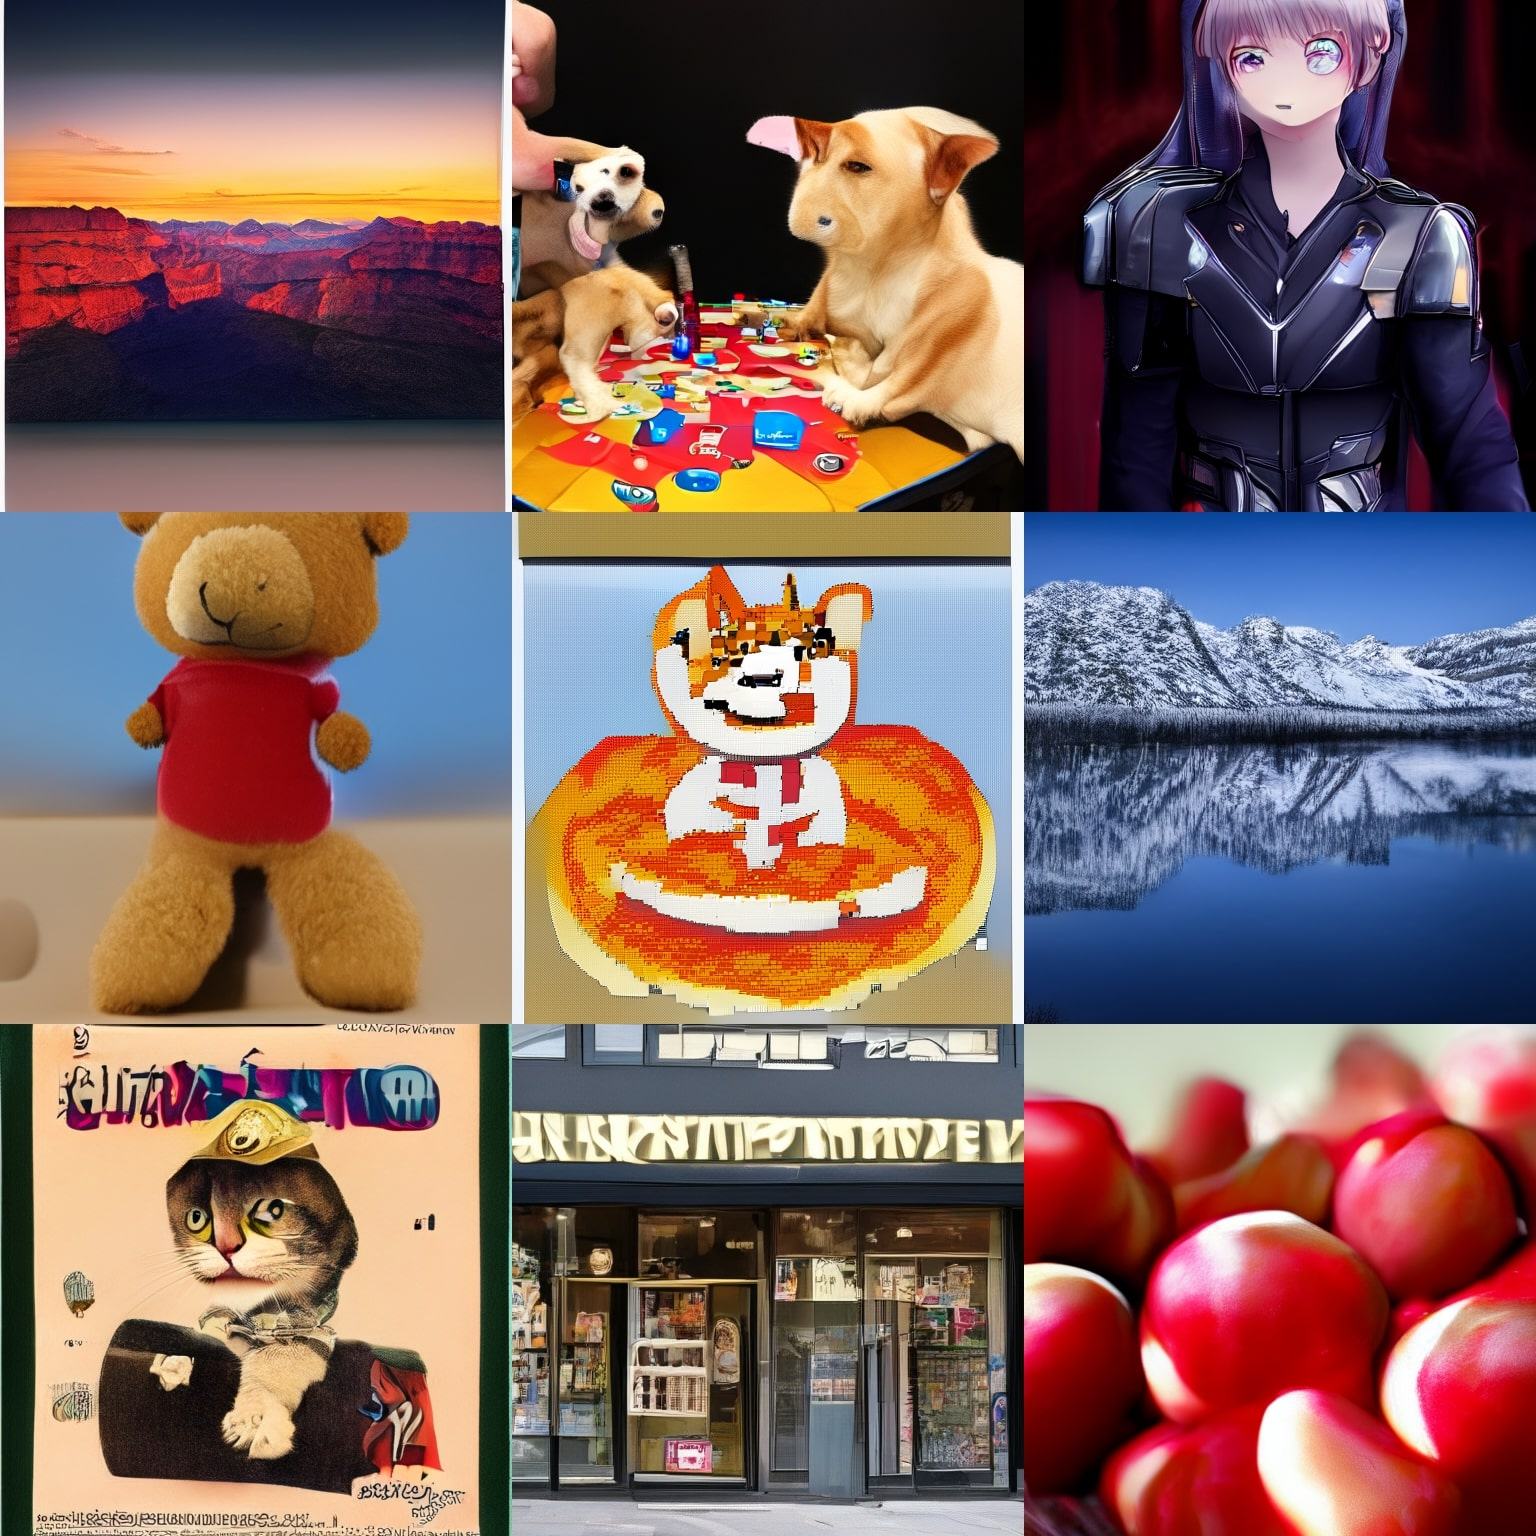
\includegraphics[width=\textwidth]{cp2/figures/t2i/c64.jpg}
    \caption{\texttt{39M} model}
    \end{subfigure}
    \begin{subfigure}[b]{0.32\textwidth}
    \centering
    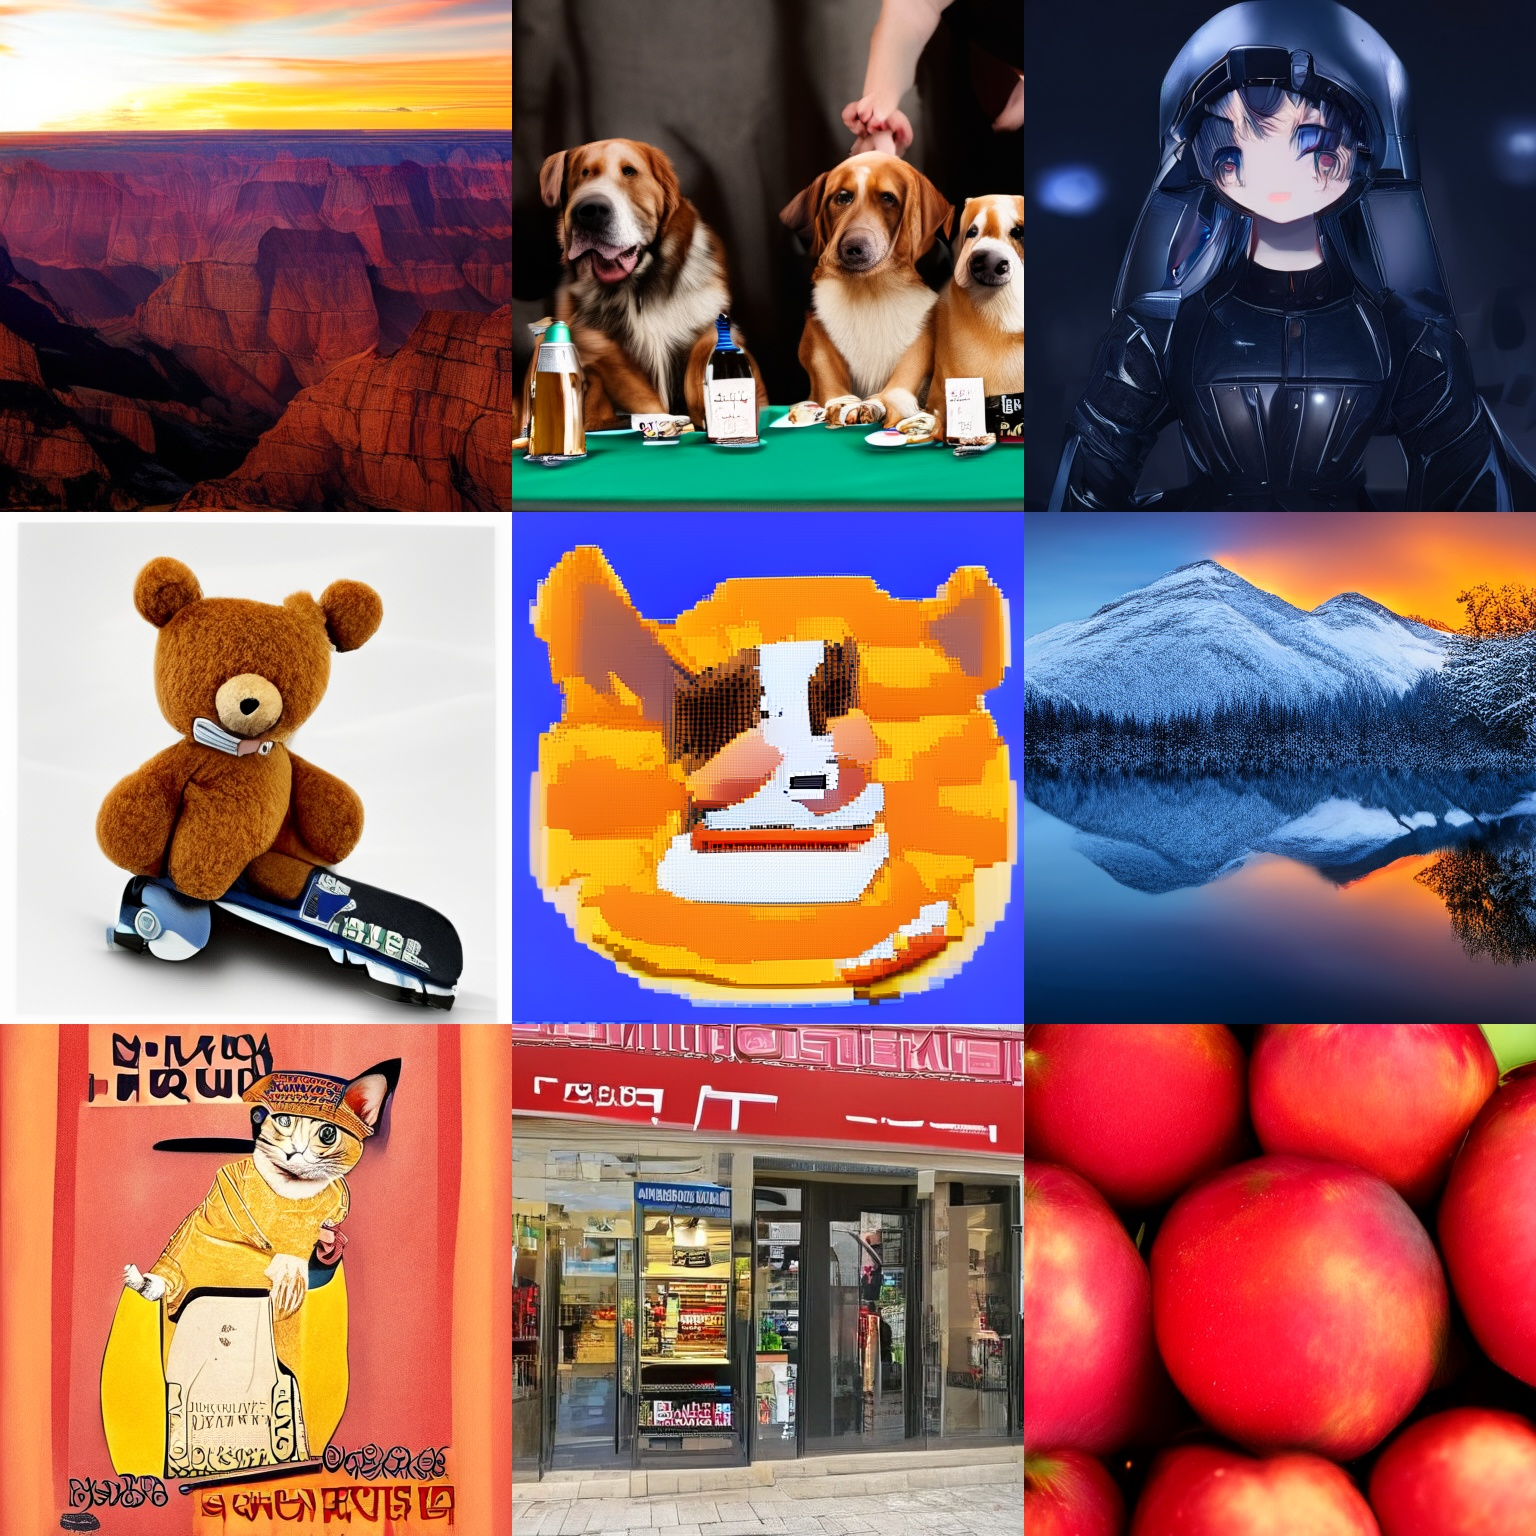
\includegraphics[width=\textwidth]{cp2/figures/t2i/c96.jpg}
    \caption{\texttt{83M} model}
    \end{subfigure}
    \begin{subfigure}[b]{0.32\textwidth}
    \centering
    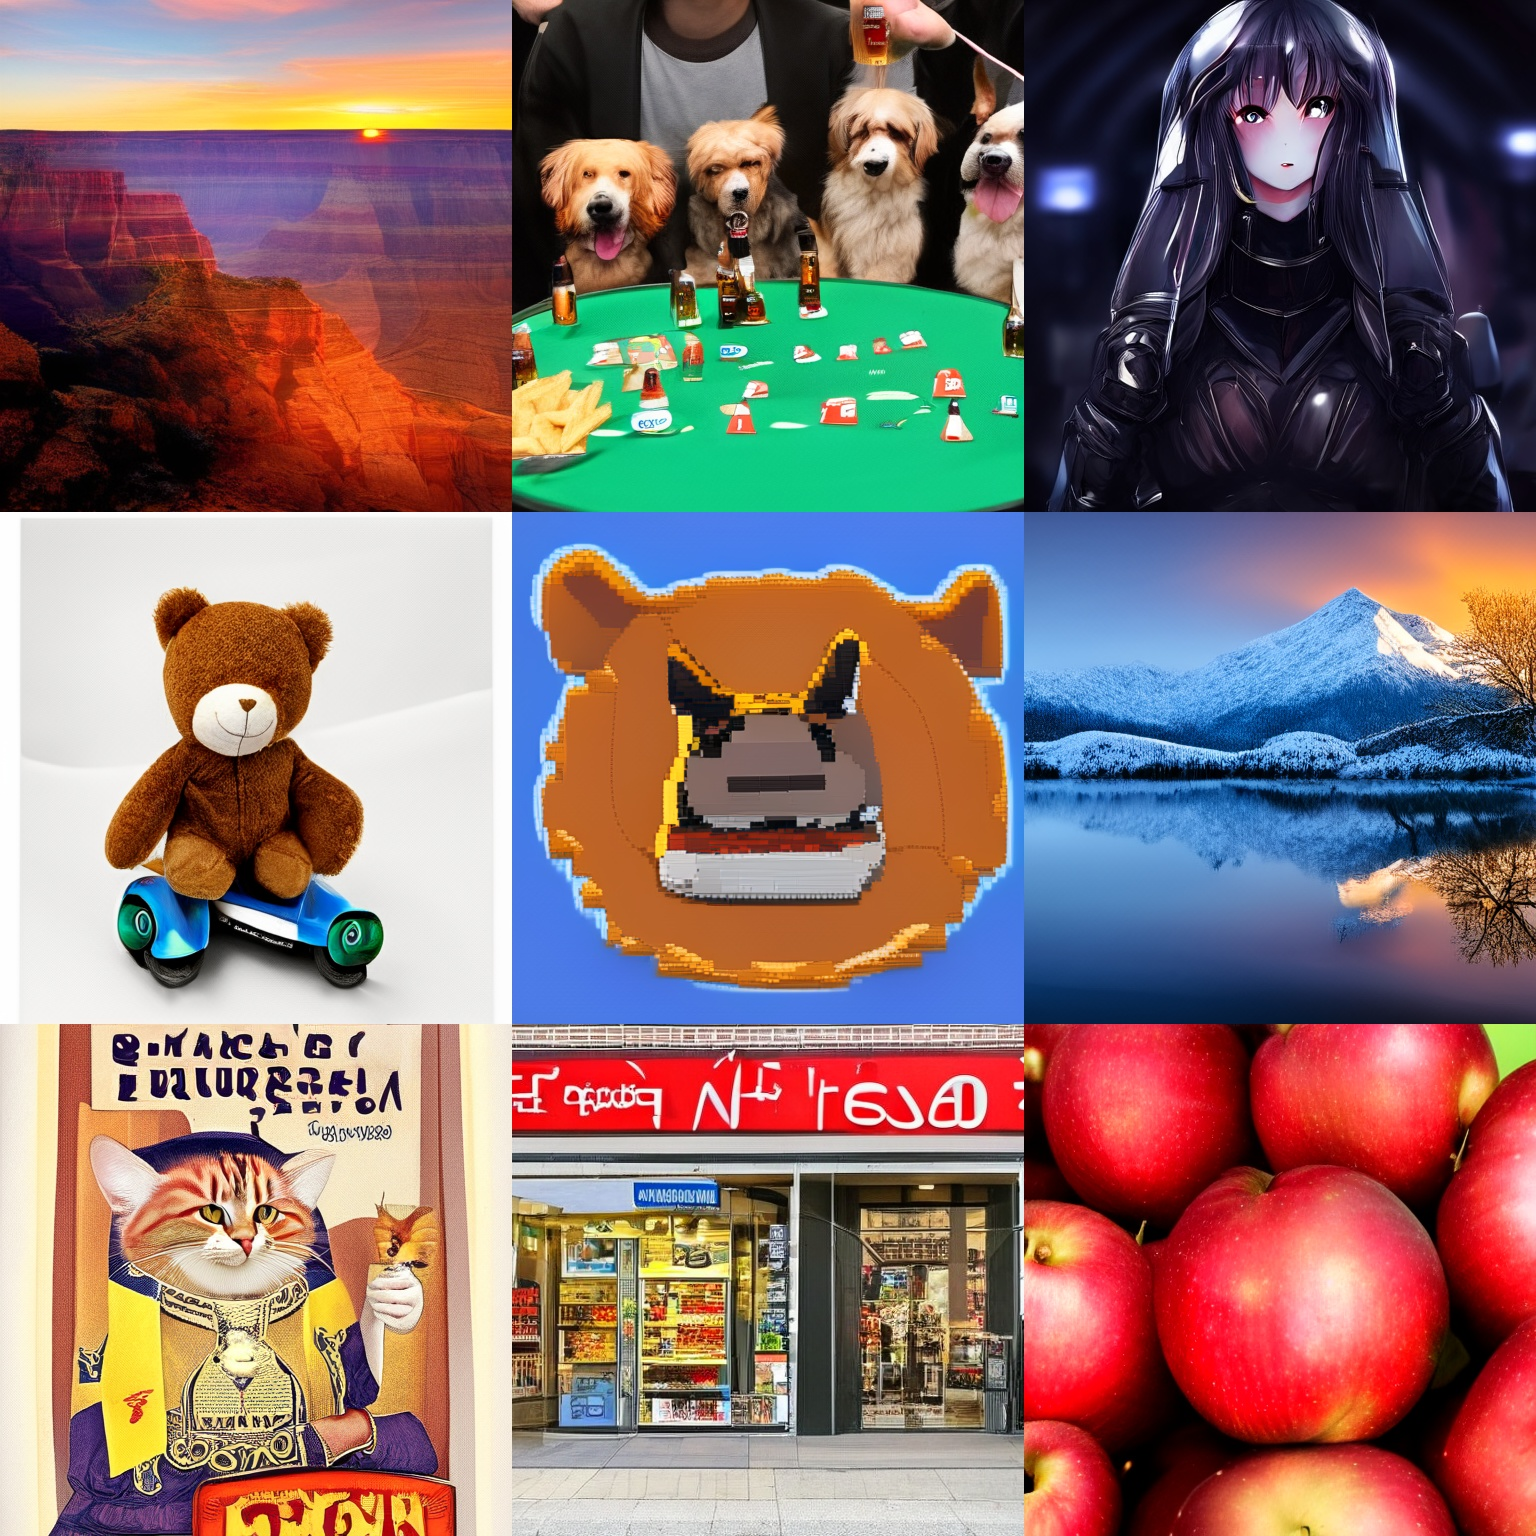
\includegraphics[width=\textwidth]{cp2/figures/t2i/c128.jpg}
    \caption{\texttt{145M} model}
    \end{subfigure}
    \hfill

    \begin{subfigure}[b]{0.32\textwidth}
    \centering
    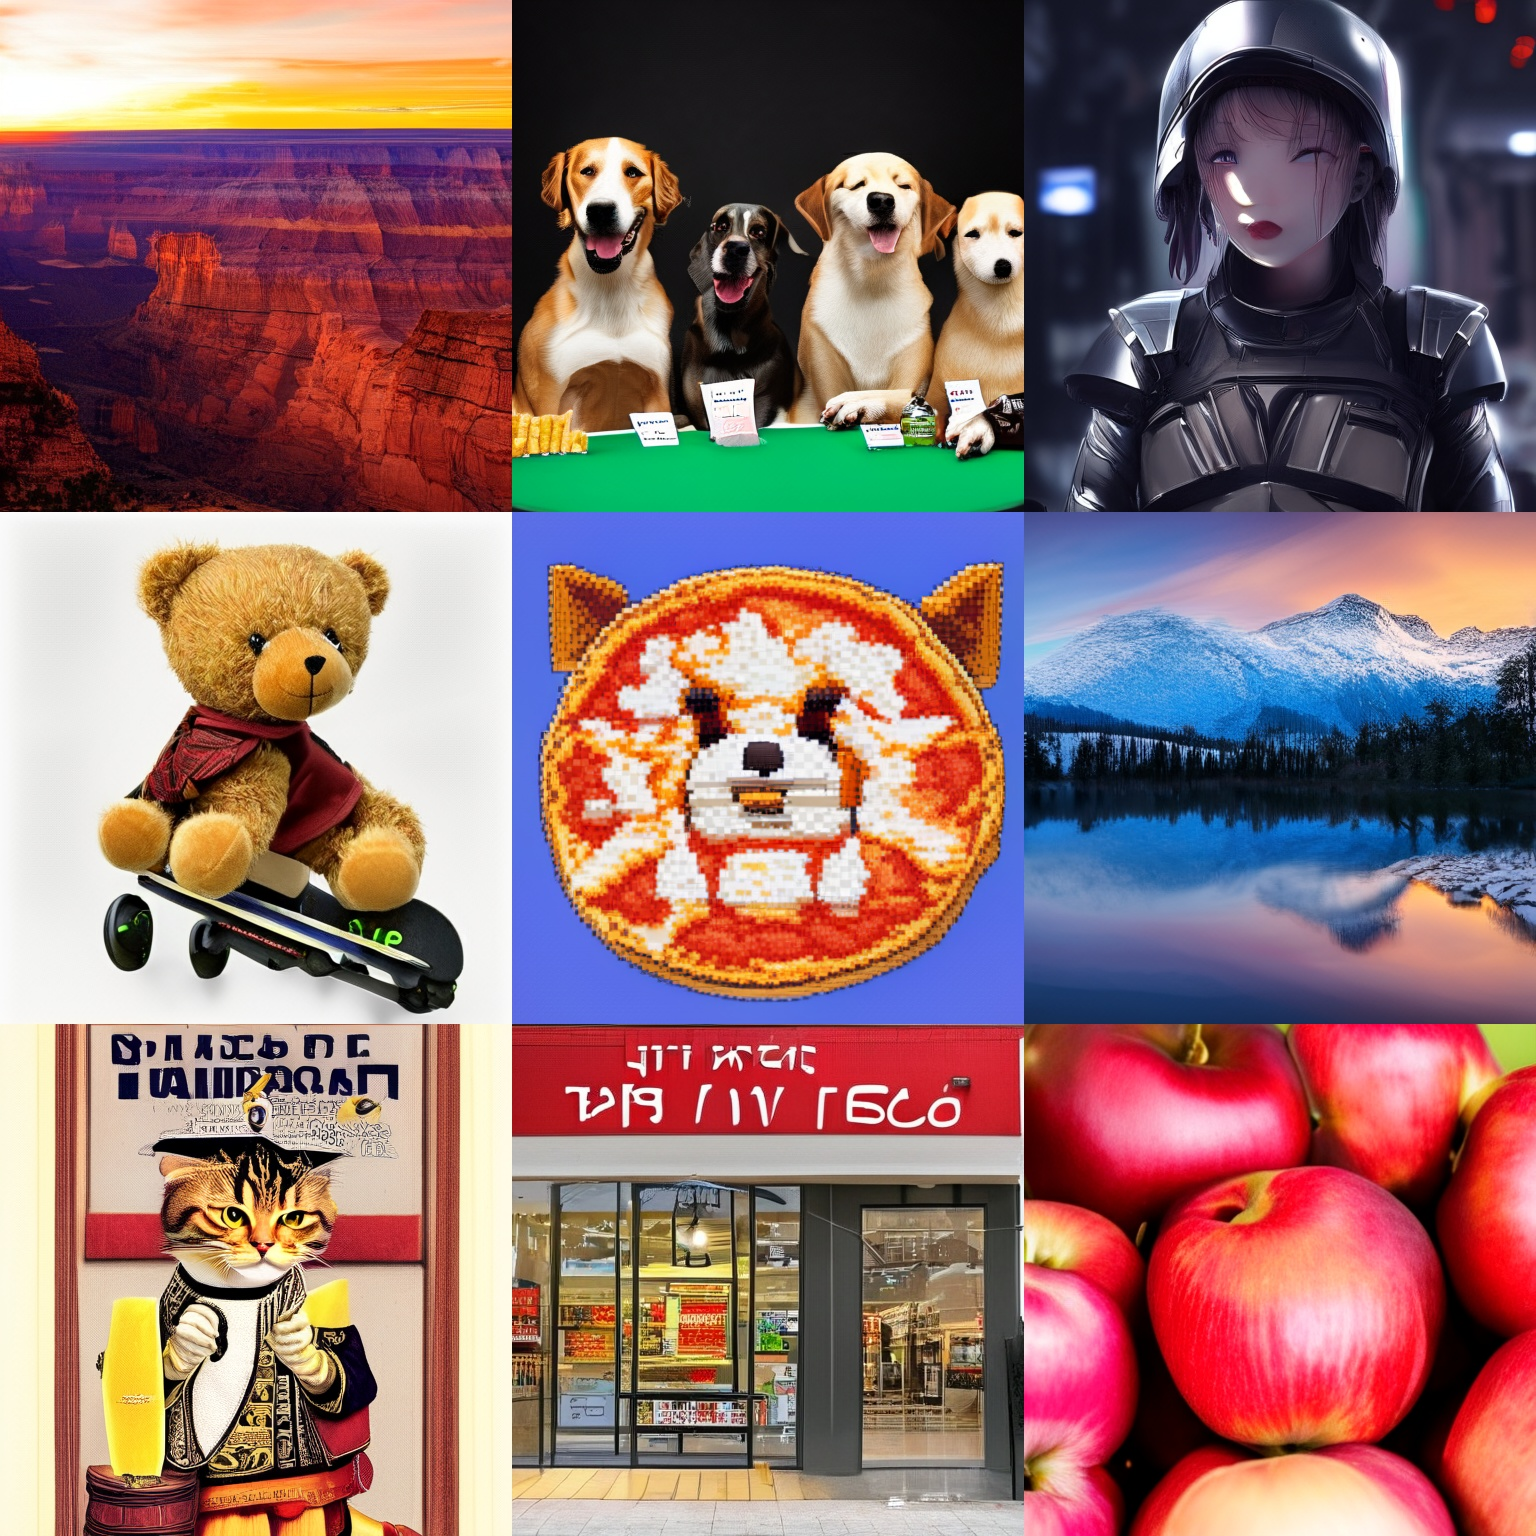
\includegraphics[width=\textwidth]{cp2/figures/t2i/c160.jpg}
    \caption{\texttt{223M} model}
    \end{subfigure}
    \begin{subfigure}[b]{0.32\textwidth}
    \centering
    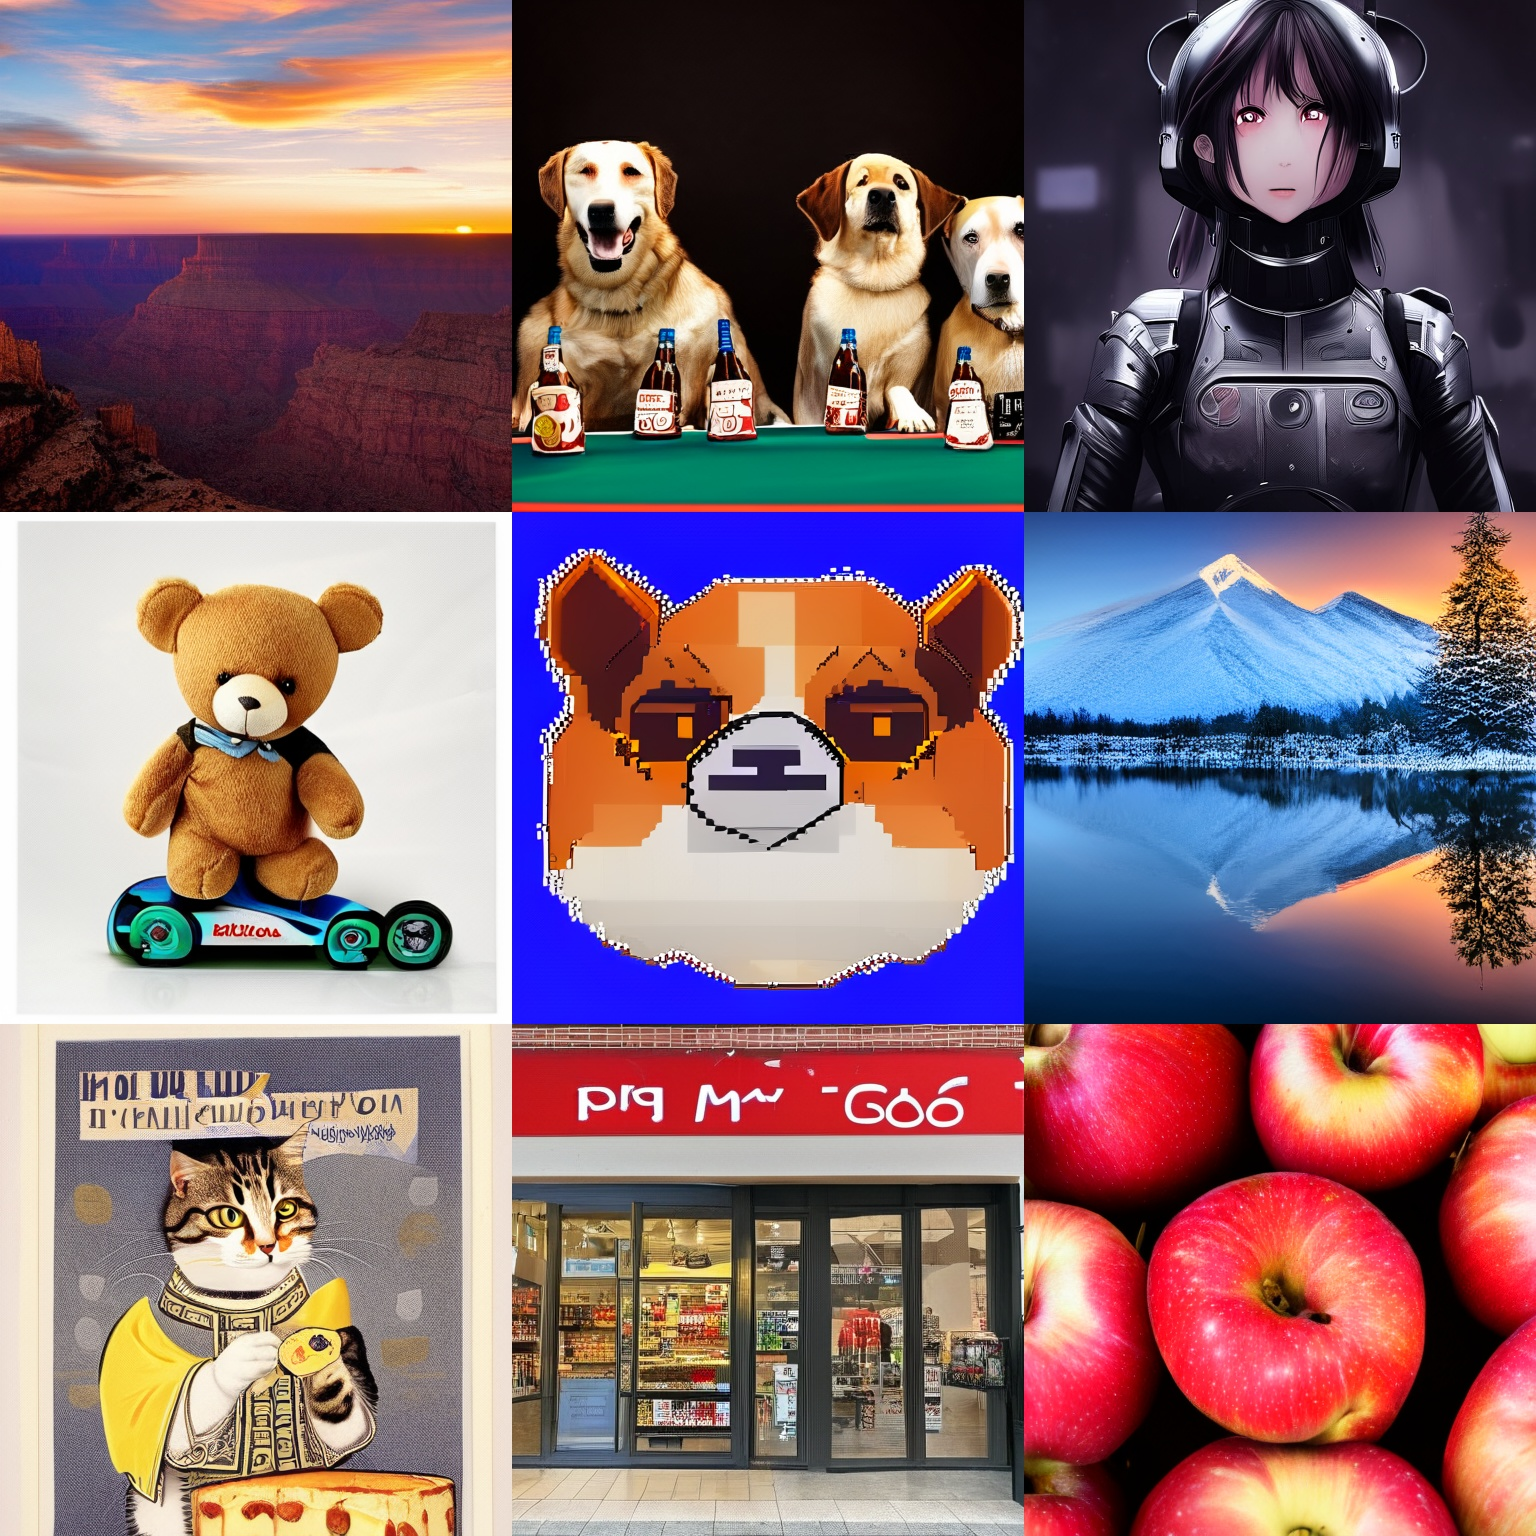
\includegraphics[width=\textwidth]{cp2/figures/t2i/c192.jpg}
    \caption{\texttt{318M} model}
    \end{subfigure}
    \begin{subfigure}[b]{0.32\textwidth}
    \centering
    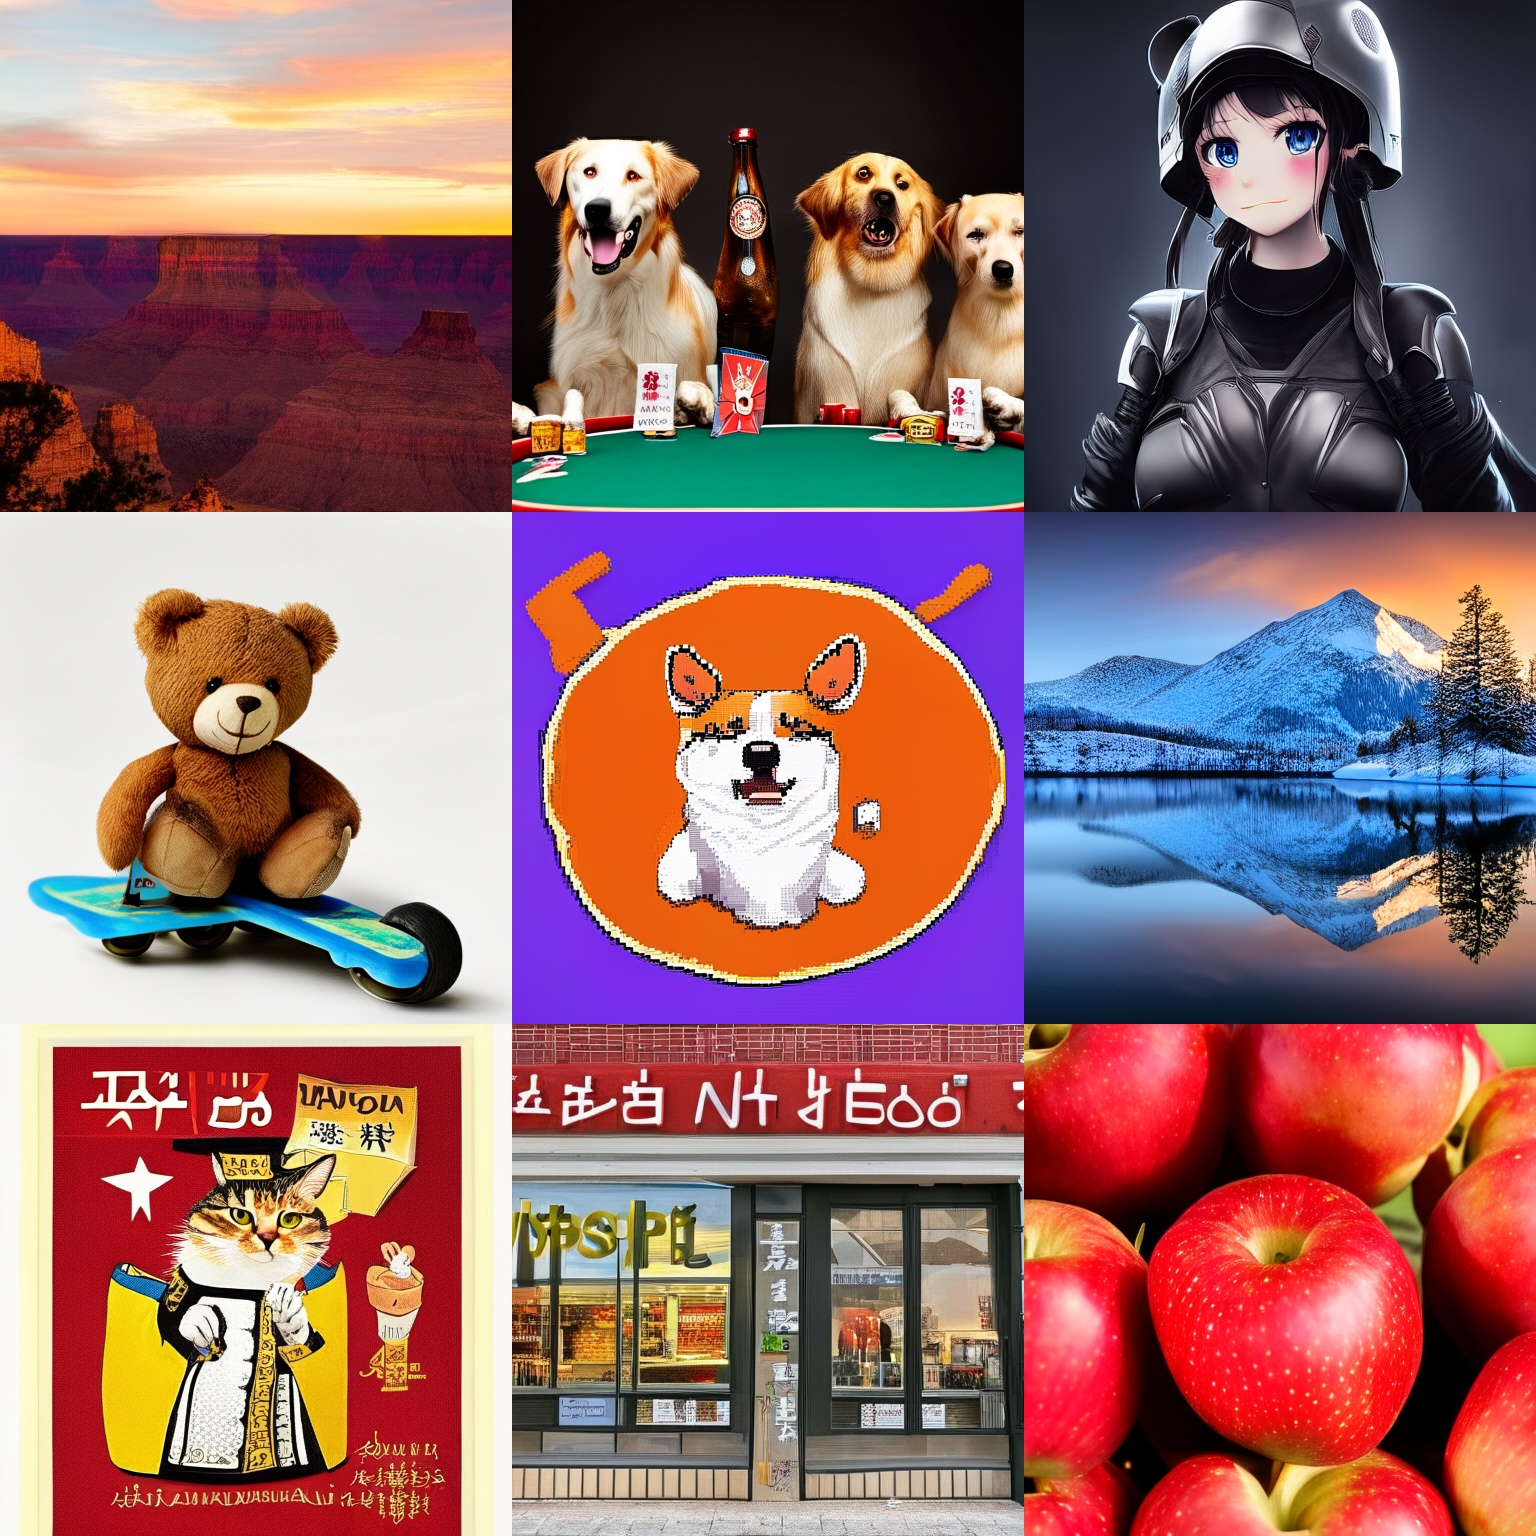
\includegraphics[width=\textwidth]{cp2/figures/t2i/c224.jpg}
    \caption{\texttt{430M} model}
    \end{subfigure}
    \hfill
    
    \begin{subfigure}[b]{0.32\textwidth}
    \centering
    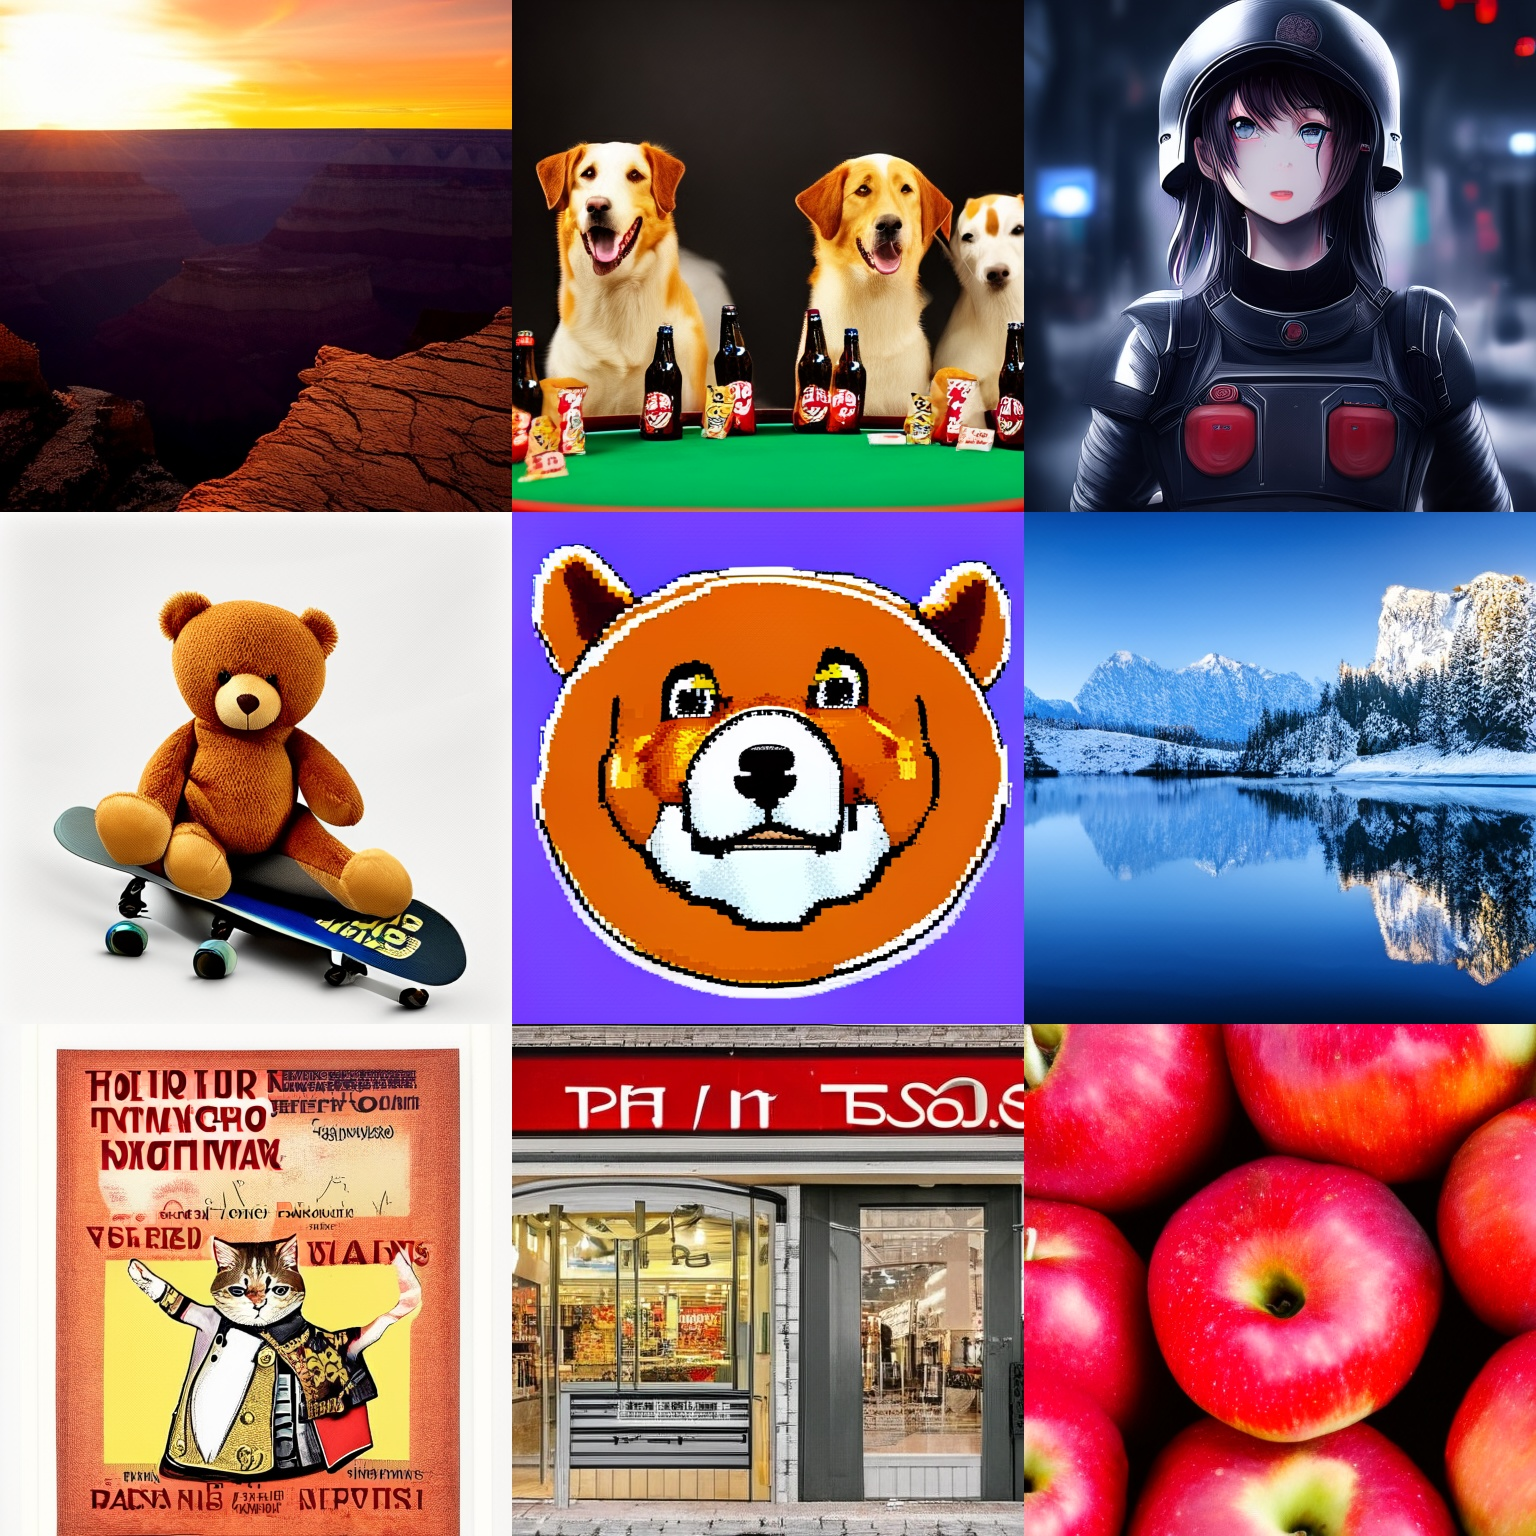
\includegraphics[width=\textwidth]{cp2/figures/t2i/c256.jpg}
    \caption{\texttt{558M} model}
    \end{subfigure}
    \begin{subfigure}[b]{0.32\textwidth}
    \centering
    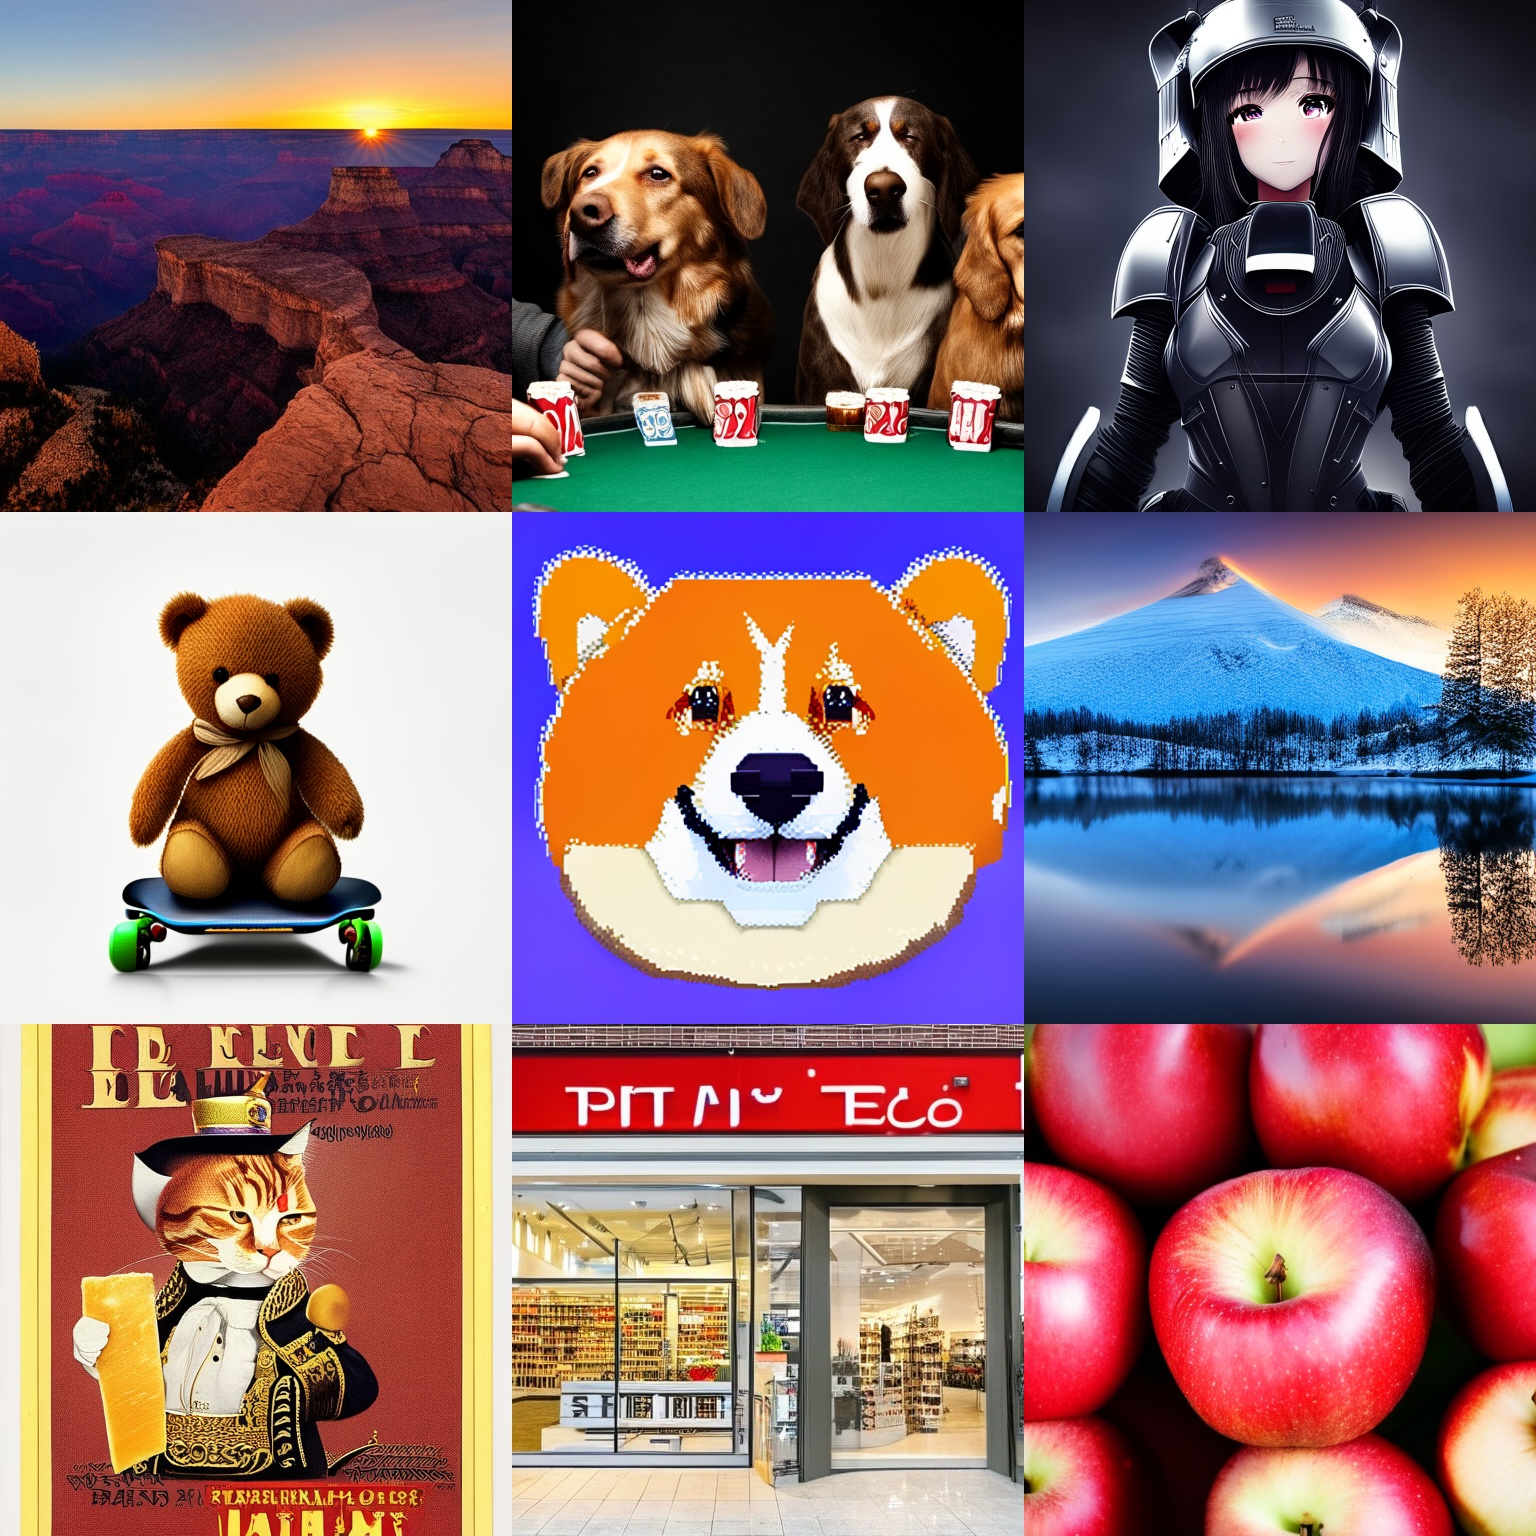
\includegraphics[width=\textwidth]{cp2/figures/t2i/c320.jpg}
    \caption{\texttt{704M} model}
    \end{subfigure}
    \begin{subfigure}[b]{0.32\textwidth}
    \centering
    
\includegraphics[width=\textwidth]{cp2/figures/t2i/c512.jpg}
    \caption{\texttt{2B} model}
    \end{subfigure}
    % \begin{subfigure}[b]{0.32\textwidth}
    % \centering
    % 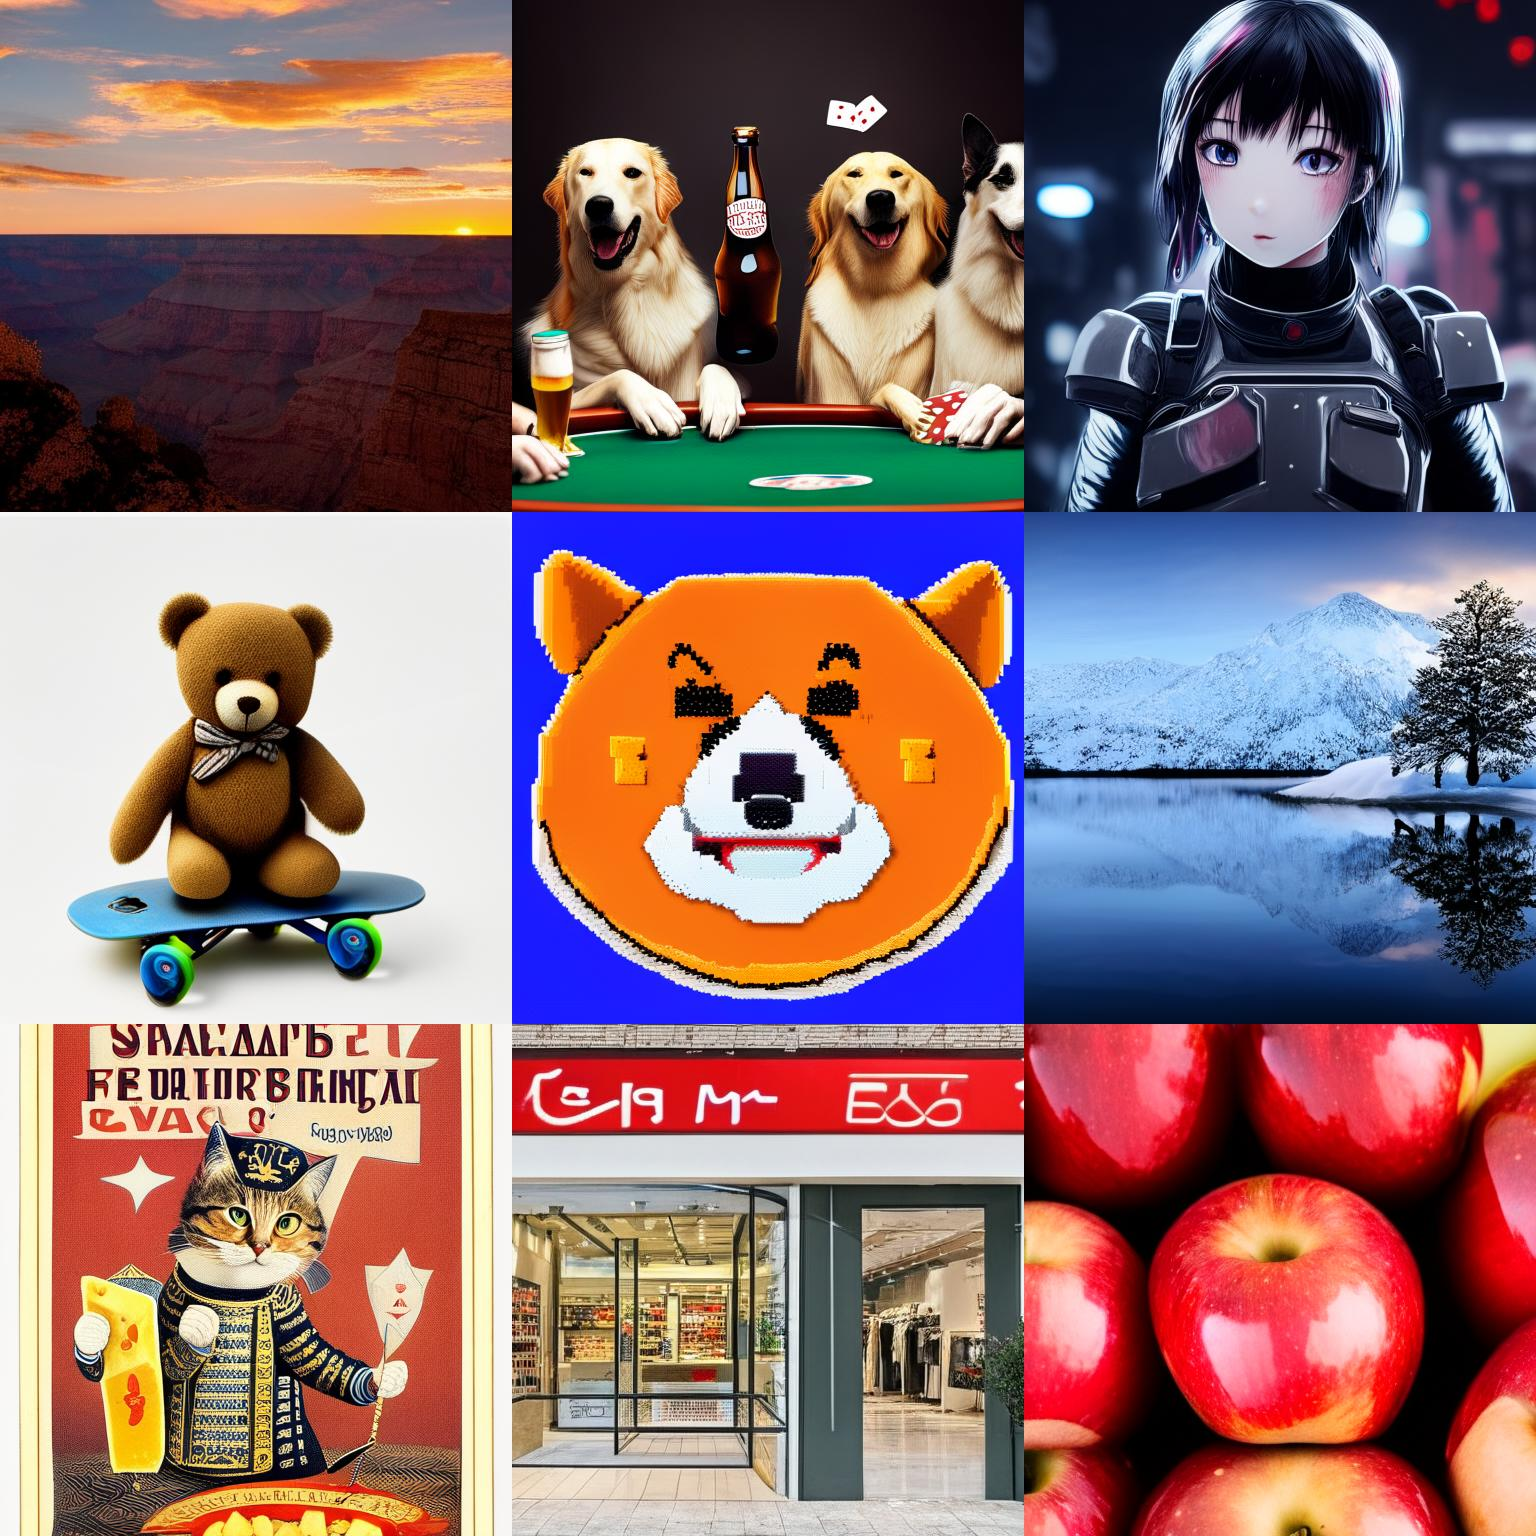
\includegraphics[width=\textwidth]{cp2/figures/t2i/c768.jpg}
    % \caption{5B model}
    % \end{subfigure}

\caption{
Text-to-image results from our scaled LDMs (\texttt{39M} - \texttt{2B}), highlighting the improvement in visual quality with increased model size (note: 39M model is the exception). All images generated using 50-step DDIM sampling and CFG rate of 7.5.
%
%An overview of text-to-image generation results for our scaled LDMs without considering the sampling efficiency, showcasing models with sizes ranging from \texttt{39M} to \texttt{2B} (due to page constraints).
%All results are generated using the same 50-step DDIM sampling.
%We find that the visual quality and details improve smoothly with larger models (except \texttt{39M} which is too small).
%
% We use representative prompts from PartiPrompts~\cite{yu2022scaling}, including \emph{``a professional photo of a sunset behind the grand canyon.''}, \emph{``Dogs sitting around a poker table with beer bottles and chips. Their hands are holding cards.''}, \emph{`Portrait of anime girl in mechanic armor in night Tokyo.''}, \emph{``a teddy bear on a skateboard.''}, \emph{``a pixel art corgi pizza.''}, \emph{``Snow mountain and tree reflection in the lake.''}, \emph{``a propaganda poster depicting a cat dressed as french emperor napoleon holding a piece of cheese.''}, \emph{``a store front that has the word ‘LDMs’ written on it.''}, and \emph{``ten red apples.''}.
}
\label{fig:t2i_results}
\end{figure*}


\begin{figure}[t]
    \centering
    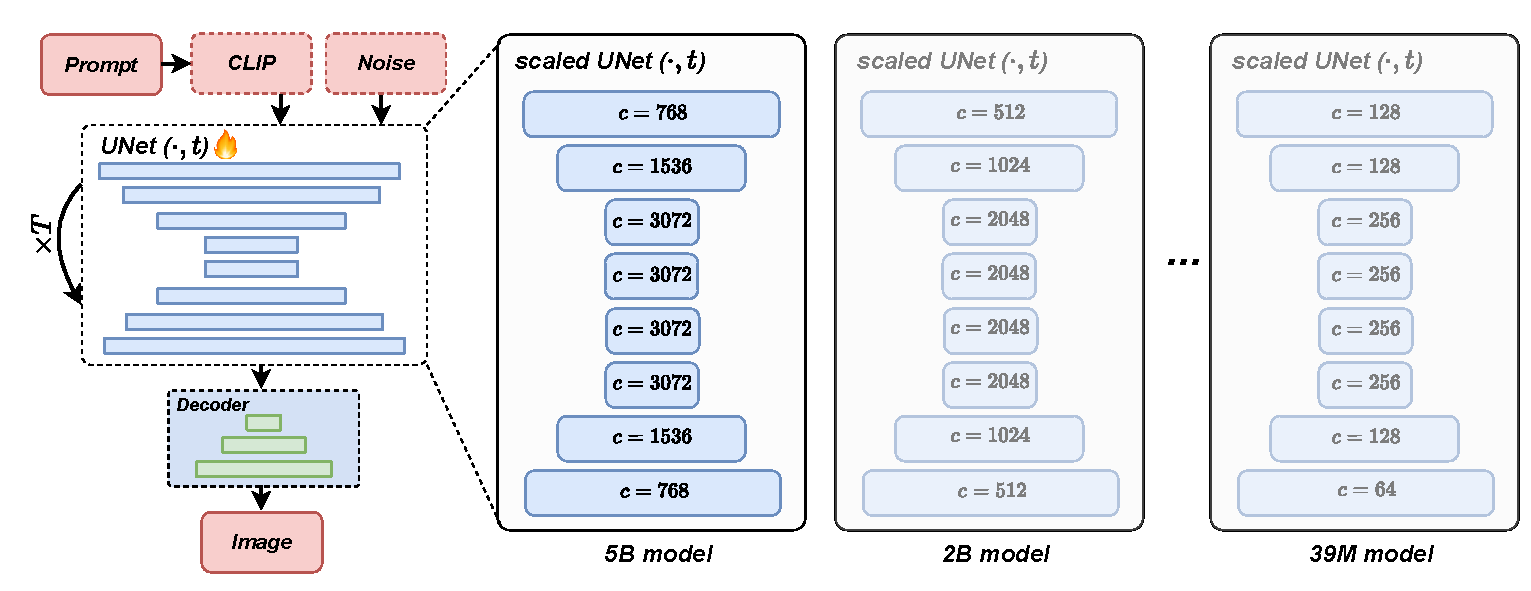
\includegraphics[width=.9\linewidth]{cp2/figures/ldm_architecture.pdf}
    % \vspace{-1\baselineskip}
    \caption{Our scaled latent diffusion models vary in the number of filters within the denoising U-Net.  Other modules remain consistent.  Smooth channel scaling (64 to 768) within residual blocks yields models ranging from \texttt{39M} to \texttt{5B} parameters. For downstream tasks requiring image input, we use an encoder to generate a latent code; this code is then concatenated with the noise vector in the denoising U-Net.}
    \label{fig:scaling_arch}
\end{figure}

\begin{figure}[!h]
    \centering
    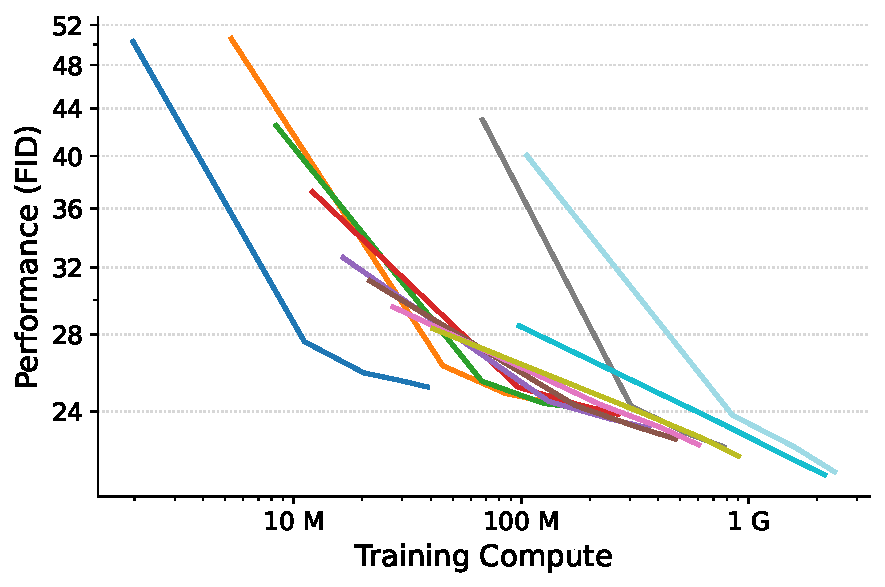
\includegraphics[height=.315\linewidth]{cp2/figures/t2i_fid_compute.pdf}
    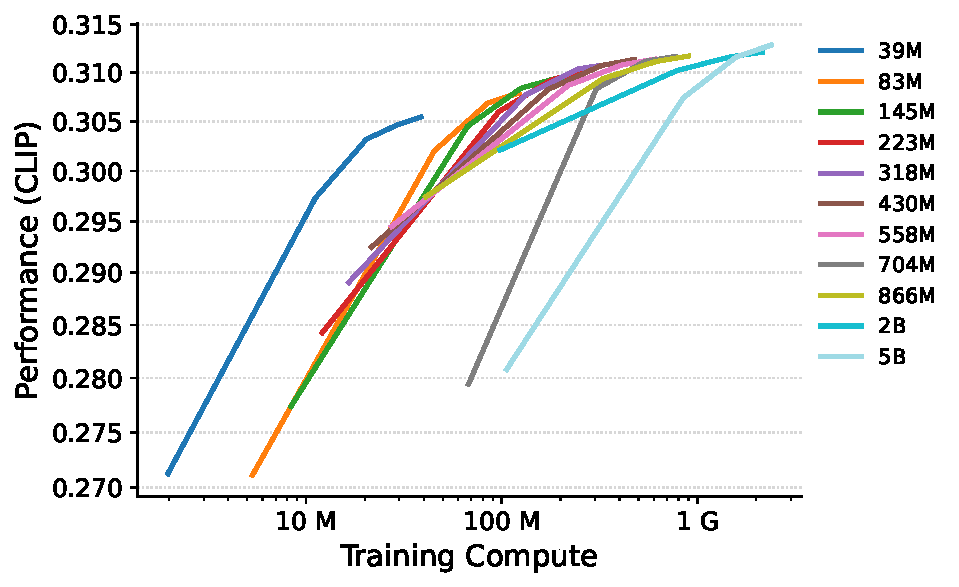
\includegraphics[height=.315\linewidth]{cp2/figures/t2i_clip_compute.pdf}
    \caption{In text-to-image generation using 50-step DDIM sampling and CFG rate of 7.5, we observe consistent trends across various model sizes in how quality metrics (FID and CLIP scores) relate to training compute (\ie, the total GFLOPS spend on training). 
    Under moderate training resources, training compute is the most relevant factor dominating quality.
    }
    \label{fig:t2i_compute}
\end{figure}

\section{Scaling LDMs}

% However, these models have been thoroughly explored and are shown to be less redundant compared with the LDMs.
% As LDMs can better performance to non-diffusion models by varying the model size.
% In this paper, we demonstrate the scaling properties of LDMs, as they can achieve 


%To smoothly scale the diffusion model size without \emph{emergence}~\cite{kaplan2020scaling, wei2022emergent}, it is crucial to ensure the generative capability is smoothly increased from small models to large models.
%We empirically show that increasing the number of filters in each residual block, while keeping the other architecture elements the same, results in smooth scaling.
%
We developed a family of powerful Latent Diffusion Models (LDMs) built upon the widely-used \texttt{866M} Stable Diffusion v1.5 standard~\cite{rombach2022high}\footnote{We adopted SD v1.5 since it is among the most popular diffusion models \url{https://huggingface.co/models?sort=likes}.}. The denoising UNet of our models offers a flexible range of sizes, with parameters spanning from \texttt{39M} to \texttt{5B}.
%
%We built a family of LDMs based on the de-facto standard, i.e., Stable Diffusion v1.4~\cite{rombach2022high}\footnote{We adopted SD v1.4 since it is the most popular diffusion models \url{https://huggingface.co/models?sort=likes}.}, spanning  a range of model size with parameters from \texttt{39M} up to \texttt{5B}.
We incrementally increase the number of filters in the residual blocks while maintaining other architecture elements the same, enabling a predictably controlled scaling.
%
Table~\ref{tab:scaling_config} shows the architectural differences among our scaled models.
%
We also provide the relative cost of each model against the baseline model.
Fig.~\ref{fig:scaling_arch} shows the architectural differences during scaling.
Models were trained using the web-scale aesthetically filtered text-to-image dataset, \ie, WebLI~\cite{chen2022pali}.
% Models were trained using internal data sources with about 600 million aesthetically-filtered text-to-image pairs.
%~\cite{chen2022pali}.
%This dataset consists of 631 million high-quality text-image pairs, being large enough to avoid overfitting the largest tested model (5B parameters).
All the models are trained for 500K steps, batch size 2048, and learning rate 1e-4.
This allows for all the models to have reached a point where we observe diminishing returns.
Fig.~\ref{fig:t2i_results} demonstrates the consistent generation capabilities across our scaled models. We used the common practice of 50 sampling steps with the DDIM sampler, 7.5 classifier-free guidance rate, for text-to-image generation. The visual quality of the results exhibits a clear improvement as model size increases.

In order to evaluate the performance of the scaled models, we test the text-to-image performance of scaled models on the validation set of COCO 2014~\cite{lin2014microsoft} with 30k samples.
For downstream performance, specifically real-world super-resolution, we test the performance of scaled models on the validation of DIV2K with 3k randomly cropped patches, which are degraded with the RealESRGAN degradation~\cite{wang2021real}.



% \begin{figure}[t]
%     \centering
%     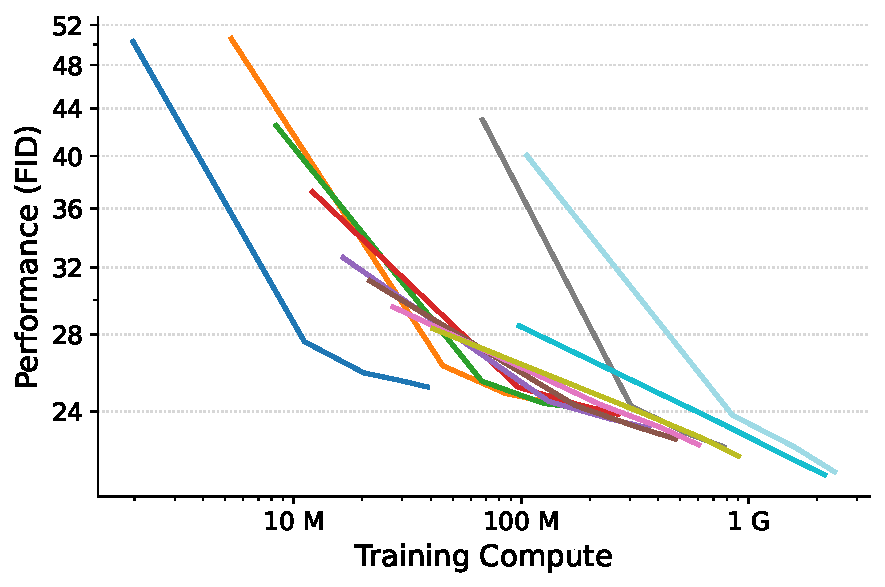
\includegraphics[height=.315\linewidth]{cp2/figures/t2i_fid_compute.pdf}
%     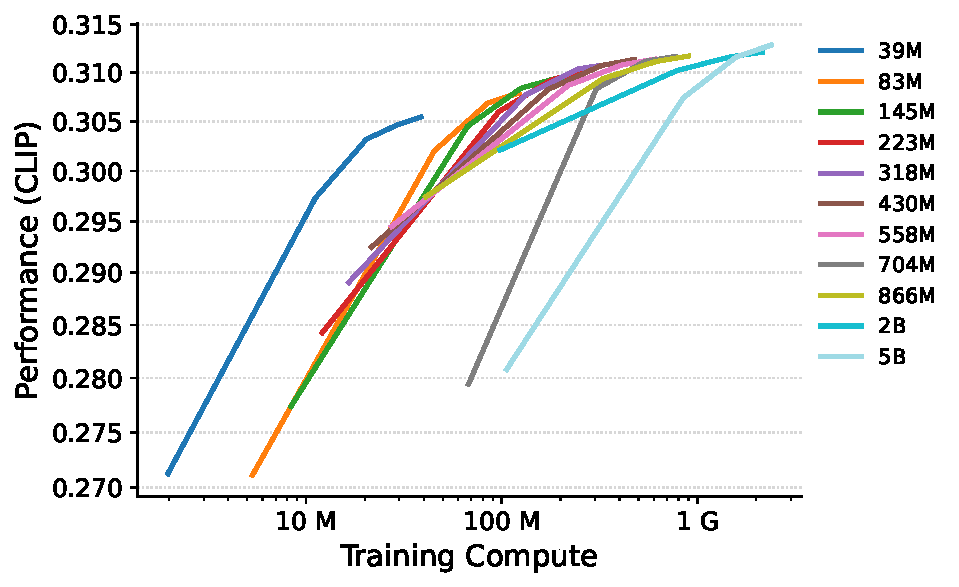
\includegraphics[height=.315\linewidth]{cp2/figures/t2i_clip_compute.pdf}
%     \caption{In text-to-image generation, we observe consistent trends across various model sizes in how quality metrics (FID and CLIP score) relate to training compute (\ie, the product of training steps and model GFLOPS). Under moderate training resources ($<1G$) training compute is the most relevant factor dominating quality. When training compute is unlimited (e.g., $\ge1G$), larger models ($>700M$) lead to superior performance.
%     %
%     Due to its massive size, the $5B$ model cannot be trained on a single TPU.  Therefore, model parallelism techniques are necessary; however, these strategies inherently introduce some accuracy trade-offs compared to training smaller models on a single device.}
%     \label{fig:t2i_compute}
%     \vspace{-1\baselineskip}
% \end{figure}

\subsection{Training compute scales text-to-image performance}
\label{sec:scalingt2i}

% \begin{table}[t]
% \centering
% \small
% \setlength{\tabcolsep}{4pt}

% \resizebox{\linewidth}{!}{
% \begin{tabular}{cccccccccccc}
% \toprule
% \textbf{Model} & \texttt{39M} & \texttt{83M} & \texttt{145M} & \texttt{223M} & \texttt{318M} & \texttt{430M} & \texttt{558M} & \texttt{704M} & \texttt{866M} & \texttt{2B} & \texttt{5B} \\
% \midrule

% \bottomrule
% \end{tabular}
% }
% \vspace{.5em}
% \caption{Text-to-image performance for our scaled LDMs (\texttt{39M}-\texttt{5B}). Larger models consistently achieve better FID score, a similar trend as seen in real image super-resolution (left panel of Figure~\ref{fig:sr_compute}).
% \caption{
% We demonstrate that the aforementioned trend between downstream performance and model size is mainly determined by the generative performance of pretrained LDMs. The performance of pretrained LDMs significantly depends on the model size, as they are pretrained with the same number of iterations.
% }
%\caption{
%We analyze the role of text-to-image pretraining in the FID/LPIPS inconsistency seen in Figure~\ref{fig:sr_compute}. Larger models consistently achieve better FID in both super-resolution and text-to-image generation ( (left panel of Figure~\ref{fig:sr_compute})). This highlights pretraining's impact on generative performance (FID), but lesser influence on distortion (LPIPS), leading to the observed divergence.

%We show the text-to-image performance of the pretraining used in super-resolution for explaining the inconsistency in Figure~\ref{fig:sr_compute}.
%Specifically, the generative performance FID (left panel of Figure~\ref{fig:sr_compute}) in super-resolution has the similar trend as the generative performance FID in text-to-image, where the larger model achieves better performance.
%The similar trend suggests that the generative performance FID of super-resolution is denominated by the pretraining, while the pretraining has less effects on the distortion performance LPIPS, and hence these two metrics show inconsistency.
% }
% \label{tab:t2i}
% \vspace{-1.5\baselineskip}
% \end{table}


We find that our scaled LDMs, across various model sizes, exhibit similar trends in generative performance relative to training compute cost, especially after training stabilizes, which typically occurs after 200K iterations.
These trends demonstrate a smooth scaling in learning capability between different model sizes.
% which allows us to discuss their sampling efficiency without involving the phenomenon of emergence, typically observed only in larger models.
To elaborate, Fig.~\ref{fig:t2i_compute} illustrates a series of training runs with models varying in size from 39 million to 5 billion parameters, where the training compute cost is quantified as the product of relative cost shown in Table~\ref{tab:scaling_config} and training iterations.
Model performance is evaluated by using the same sampling steps and sampling parameters.
%When training compute is limited, these trends suggest that the generative performance of T2I models is primarily dependent on the training compute, indicating that the scalability of LDMs is not significantly hindered by variations in model size.
In scenarios with moderate training compute (i.e., $<1G$, see Fig.~\ref{fig:t2i_compute}), the generative performance of T2I models scales well with additional compute resources. 


\begin{figure}[t]
\centering
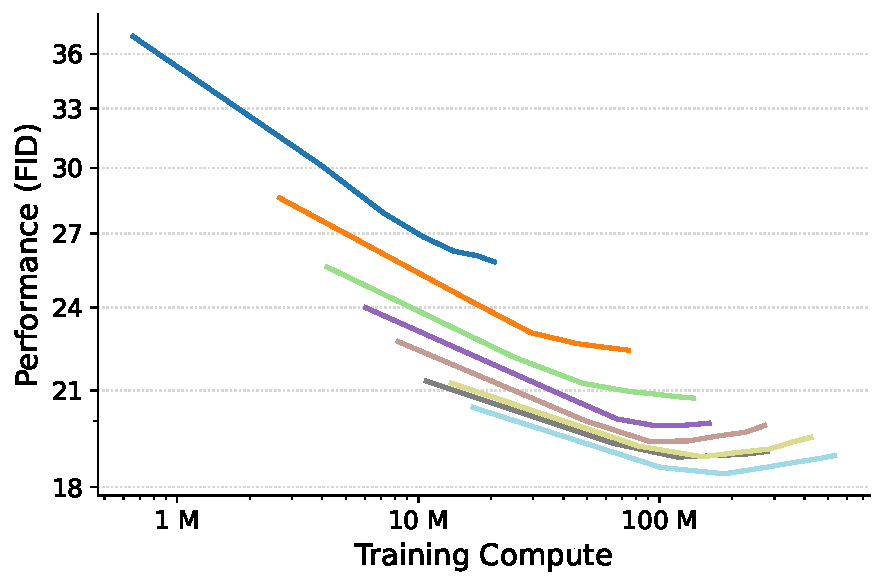
\includegraphics[height=.315\linewidth]{cp2/figures/sr_fid_compute.pdf}
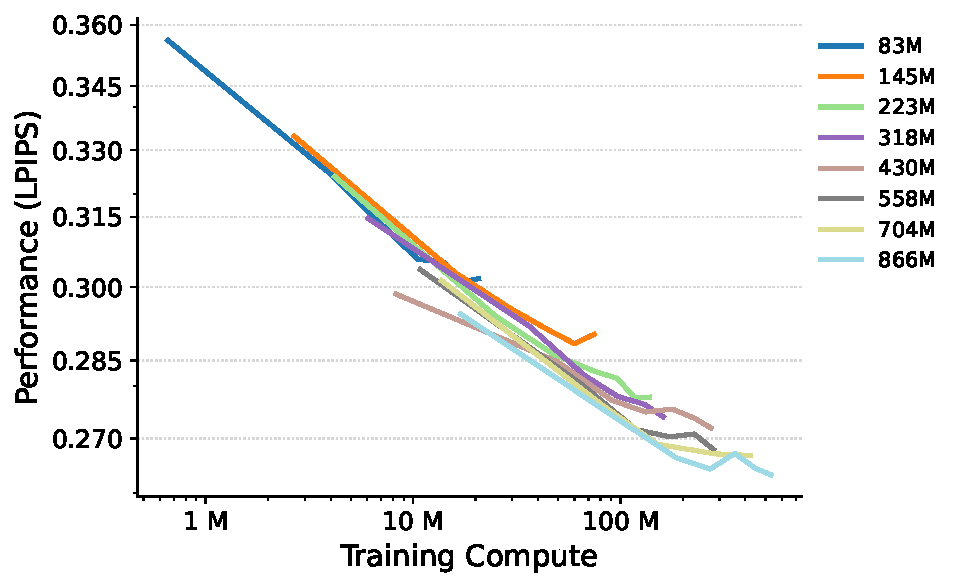
\includegraphics[height=.315\linewidth]{cp2/figures/sr_lpips_compute.pdf}
\caption{In $4\times$ real image super-resolution using 50-step DDIM sampling, FID and LPIPS scores reveal an interesting divergence. Model size drives FID score improvement, while training compute most impacts LPIPS score. Despite this, visual assessment (Fig.~\ref{fig:sr}) confirms the importance of model size for superior detail recovery (similarly as observed in the text-to-image pretraining).
}
\label{fig:sr_compute}
\end{figure}

\begin{figure}[!ht]
    \scriptsize
    \centering
    \def\xwidth{0.12\linewidth}
    \setlength{\tabcolsep}{1pt}
    \begin{tabular}[t]{c c c c c c}
    &
    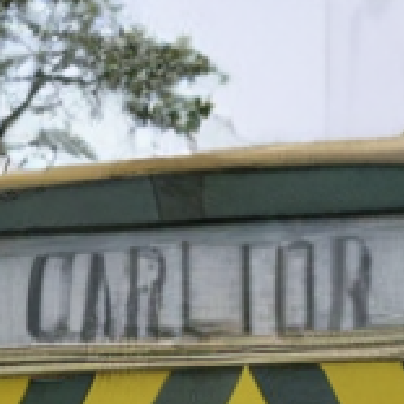
\includegraphics[width=\xwidth]{cp2/figures/sr/scaling_sr_c96_2.png} &
    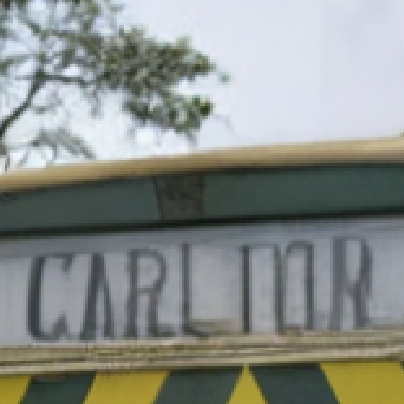
\includegraphics[width=\xwidth]{cp2/figures/sr/scaling_sr_c128_2.png} &
    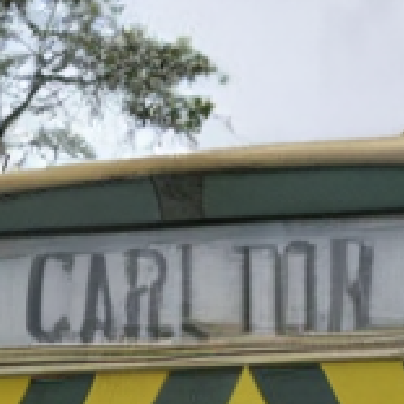
\includegraphics[width=\xwidth]{cp2/figures/sr/scaling_sr_c160_2.png} &
    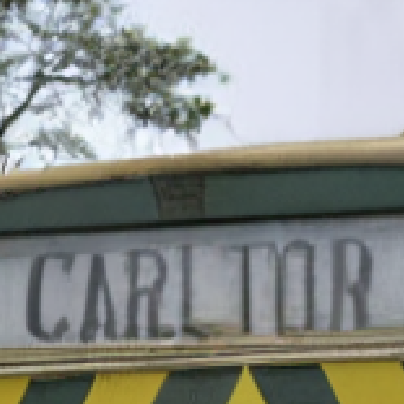
\includegraphics[width=\xwidth]{cp2/figures/sr/scaling_sr_c192_2.png} &
    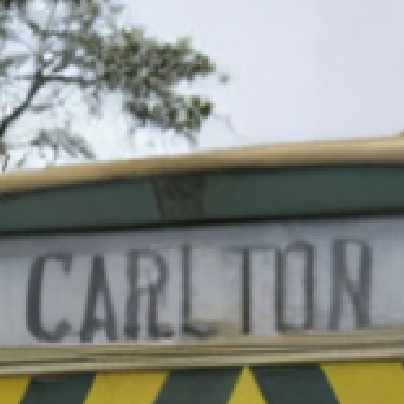
\includegraphics[width=\xwidth]{cp2/figures/sr/scaling_sr_c224_2.png}
    \\[-0.2em]
    & \scriptsize \texttt{83M} & \scriptsize \texttt{145M} & \scriptsize \texttt{223M} & \scriptsize \texttt{318M} & \scriptsize \texttt{430M}
    \\
    \multirow[t]{3}{*}{
    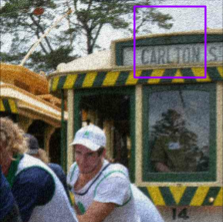
\includegraphics[width=0.2645\linewidth, height=0.2645\linewidth]{cp2/figures/sr/scaling_sr_lr_2.png}
    } &
    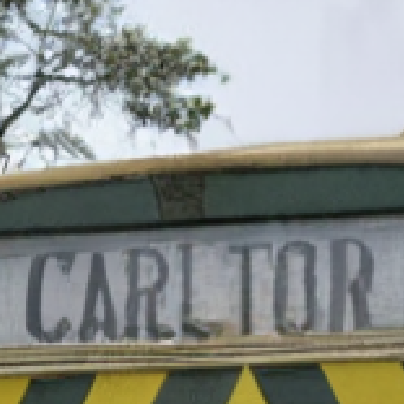
\includegraphics[width=\xwidth]{cp2/figures/sr/scaling_sr_c256_2.png} &
    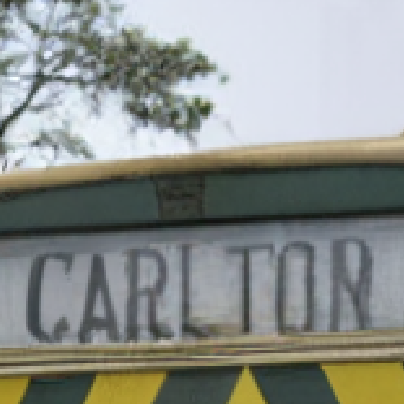
\includegraphics[width=\xwidth]{cp2/figures/sr/scaling_sr_c320_2.png} &
    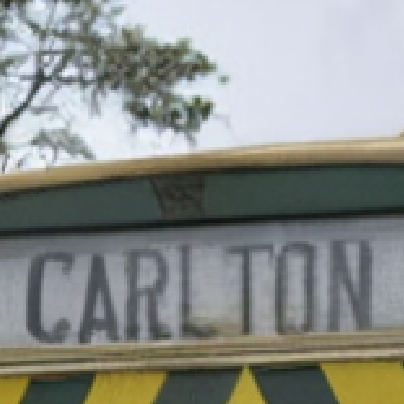
\includegraphics[width=\xwidth]{cp2/figures/sr/scaling_sr_c512_2.png} &
    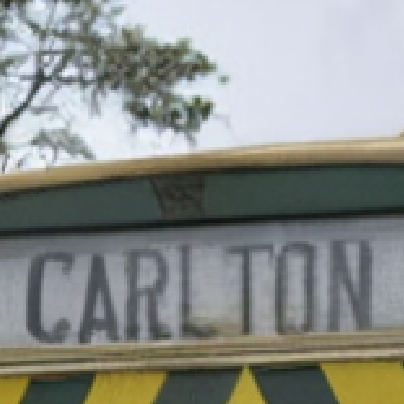
\includegraphics[width=\xwidth]{cp2/figures/sr/scaling_sr_c512_2.png} &
    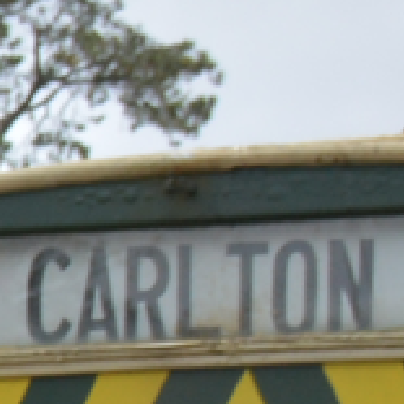
\includegraphics[width=\xwidth]{cp2/figures/sr/scaling_sr_hr_2.png}
    \\[-0.2em]
    \scriptsize LR &  \scriptsize \texttt{558M} & \scriptsize \texttt{704M} & \scriptsize \texttt{866M} & \scriptsize \texttt{2B} & \scriptsize HR
    \\
    &
    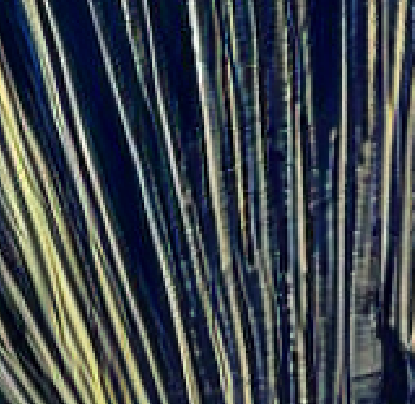
\includegraphics[width=\xwidth]{cp2/figures/sr/scaling_sr_c96_1.png} &
    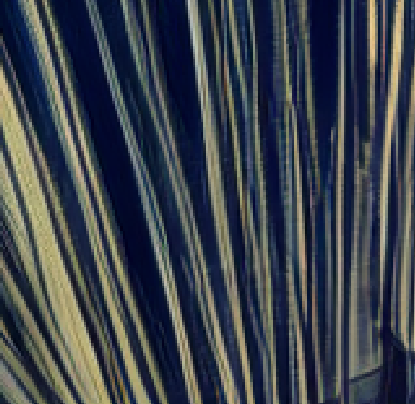
\includegraphics[width=\xwidth]{cp2/figures/sr/scaling_sr_c128_1.png} &
    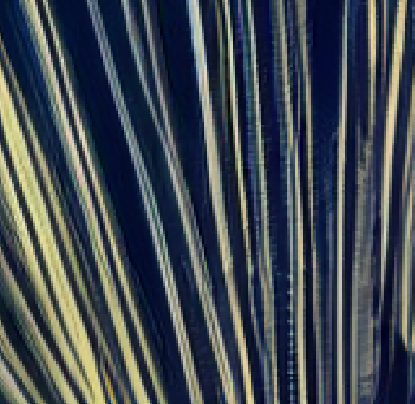
\includegraphics[width=\xwidth]{cp2/figures/sr/scaling_sr_c160_1.png} &
    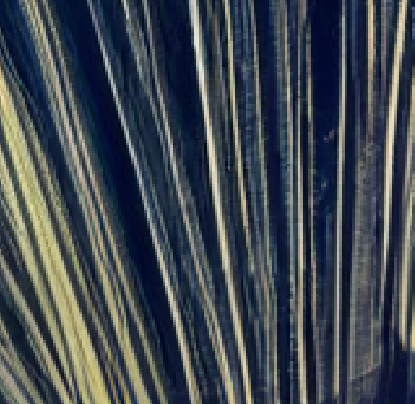
\includegraphics[width=\xwidth]{cp2/figures/sr/scaling_sr_c192_1.png} &
    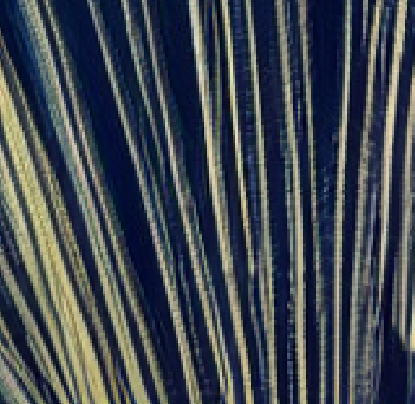
\includegraphics[width=\xwidth]{cp2/figures/sr/scaling_sr_c224_1.png}
    \\[-0.2em]
    & \scriptsize \texttt{83M} & \scriptsize \texttt{145M} & \scriptsize \texttt{223M} & \scriptsize \texttt{318M} & \scriptsize \texttt{430M}
    \\
    \multirow[t]{3}{*}{
    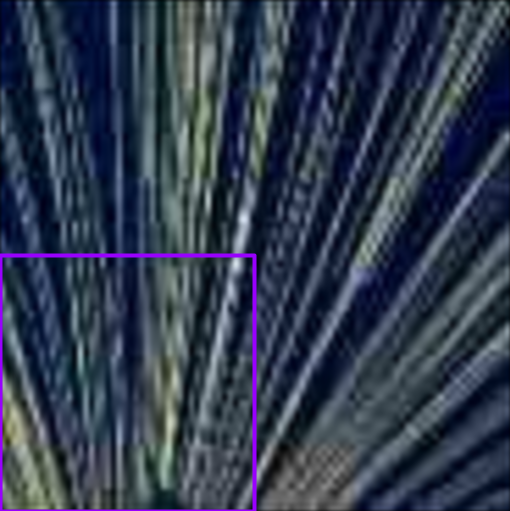
\includegraphics[width=0.26\linewidth,height=0.26\linewidth]{cp2/figures/sr/scaling_sr_lr_1.png}
    } &
    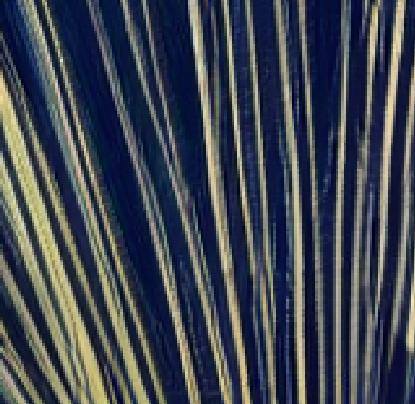
\includegraphics[width=\xwidth]{cp2/figures/sr/scaling_sr_c256_1.png} &
    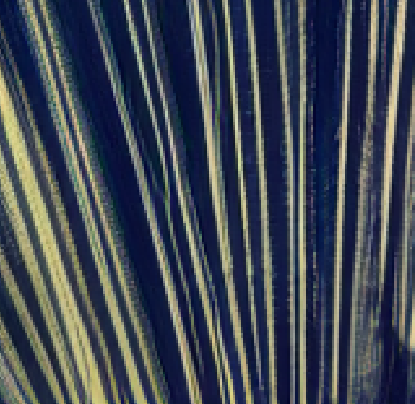
\includegraphics[width=\xwidth]{cp2/figures/sr/scaling_sr_c320_1.png} &
    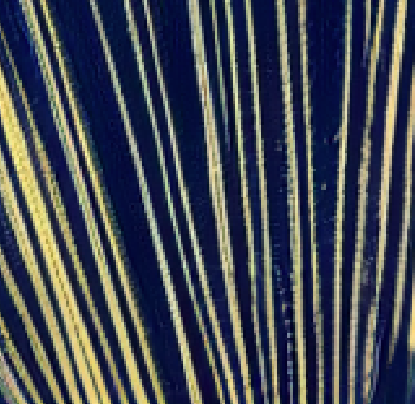
\includegraphics[width=\xwidth]{cp2/figures/sr/scaling_sr_c512_1.png} &
    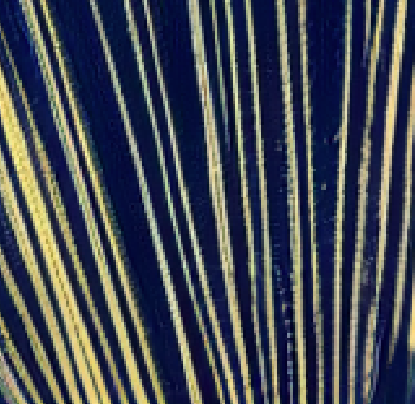
\includegraphics[width=\xwidth]{cp2/figures/sr/scaling_sr_c512_1.png} &
    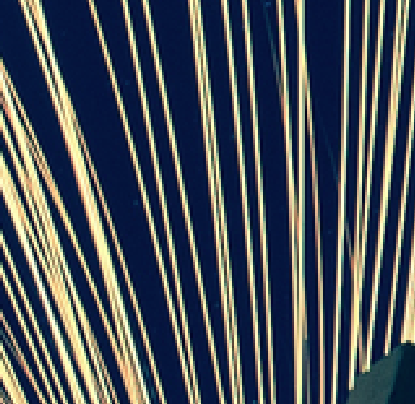
\includegraphics[width=\xwidth]{cp2/figures/sr/scaling_sr_hr_1.png}
    \\[-0.2em]
    \scriptsize LR &  \scriptsize \texttt{558M} & \scriptsize \texttt{704M} & \scriptsize \texttt{866M} & \scriptsize \texttt{2B} & \scriptsize HR
    \end{tabular}
    \caption{In 4$\times$ super-resolution using 50-step DDIM sampling, visual quality directly improves with increased model size. As these scaled models vary in pretraining performance, the results clearly demonstrate that pretraining boosts super-resolution capabilities in both quantitative (Fig~\ref{fig:sr_compute}) and qualitative ways.
    }
    %
    %In $4\times$ super-resolution, we observe that the visual quality of sampled results increases as the model size increases. The scaled models differ in pretraining performance, and thus, the results further demonstrate that pretraining scales the super-resolution performance of LDMs both quantitatively (Fig~\ref{fig:sr_compute}) and qualitatively.}
    \label{fig:sr}
\end{figure}

\begin{figure*}[!ht]
\scriptsize
    \centering
    \def\xwidth{0.135\linewidth}
    \setlength{\tabcolsep}{0.5pt}
    \begin{tabular}[t]{c c c c c}
    &
    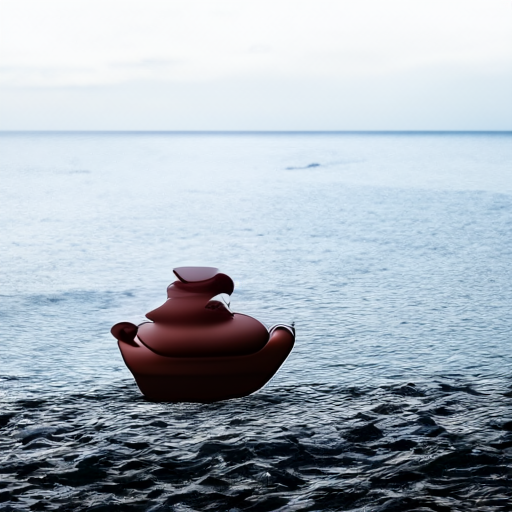
\includegraphics[width=\xwidth]{cp2/figures/dreambooth/teapot/c96_checkpoint_599.png} &
    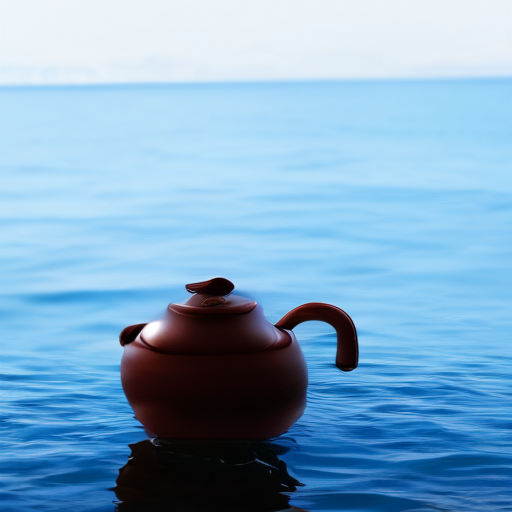
\includegraphics[width=\xwidth]{cp2/figures/dreambooth/teapot/c128_checkpoint_199.png} &
    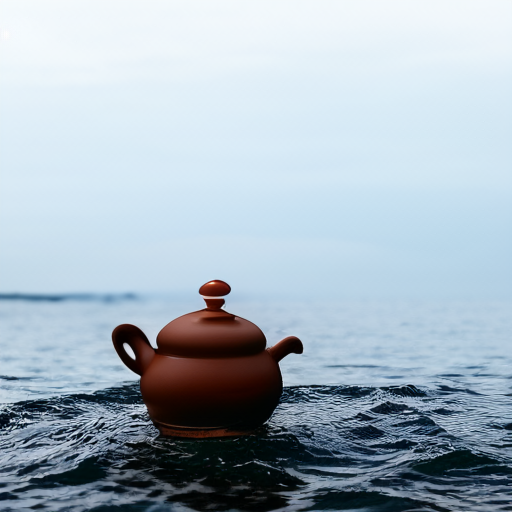
\includegraphics[width=\xwidth]{cp2/figures/dreambooth/teapot/c160_checkpoint_399.png} &
    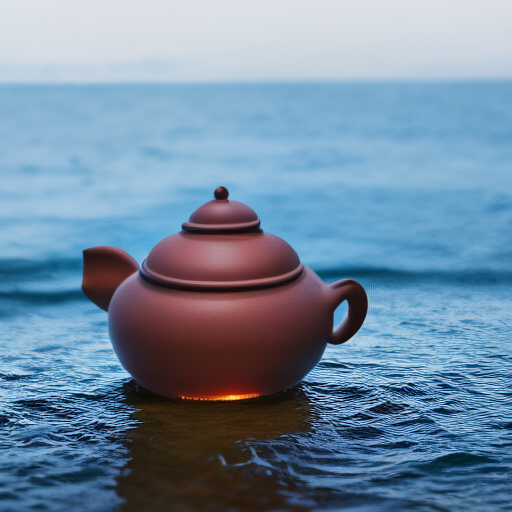
\includegraphics[width=\xwidth]{cp2/figures/dreambooth/teapot/c192_checkpoint_999.png} \\
    & \texttt{83M} & \texttt{145M} & \texttt{223M} & \texttt{318M} \\
    \multirow[t]{3}{*}{
    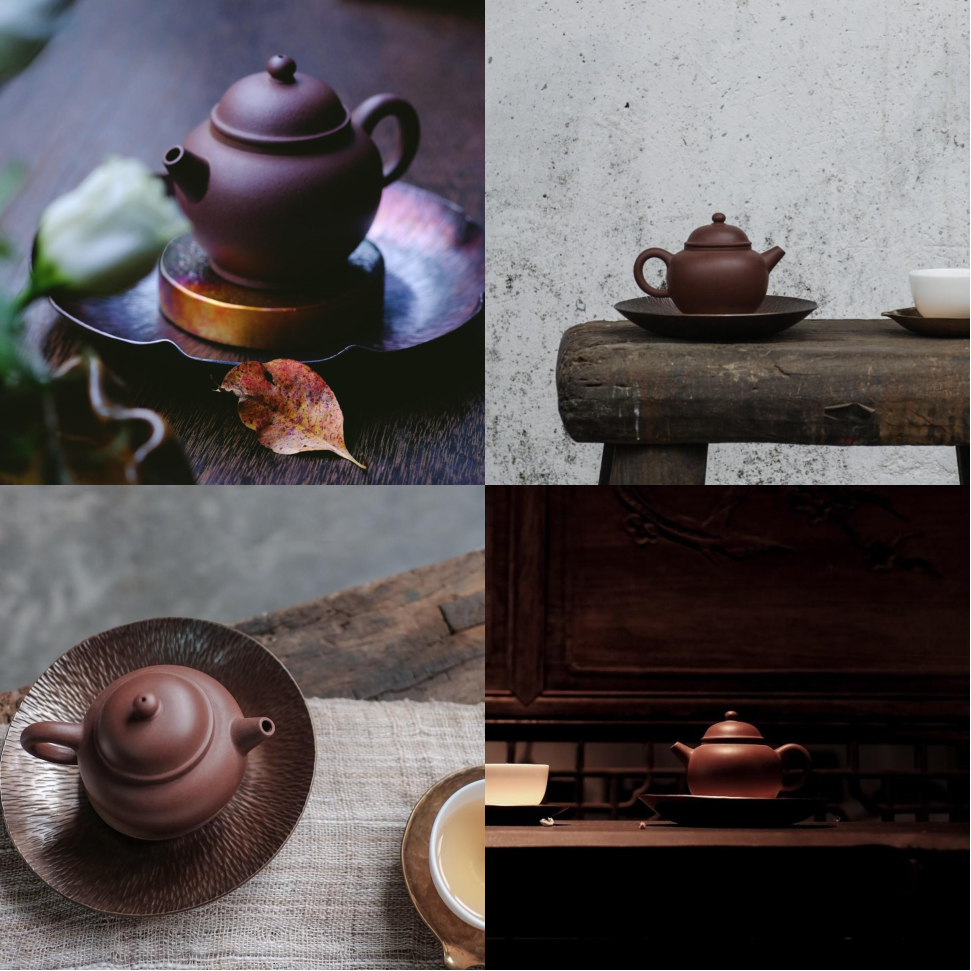
\includegraphics[width=0.3\linewidth]{cp2/figures/dreambooth/teapot/teapot.pdf}
    } &
    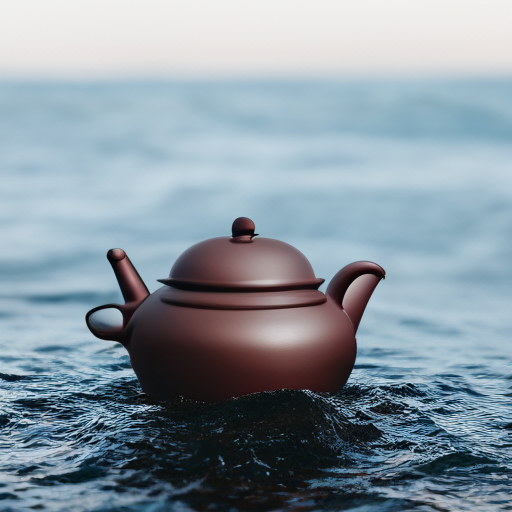
\includegraphics[width=\xwidth]{cp2/figures/dreambooth/teapot/c224_checkpoint_399.png} &
    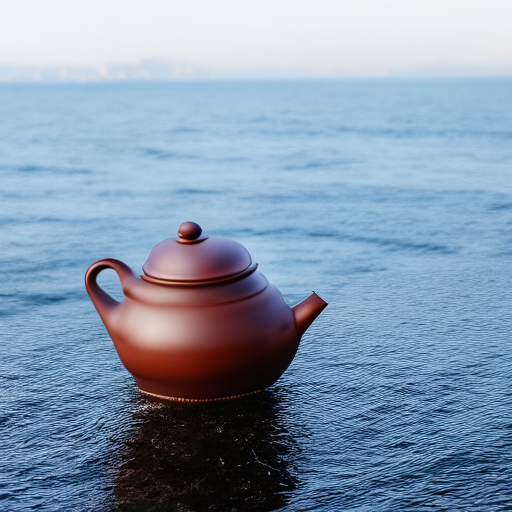
\includegraphics[width=\xwidth]{cp2/figures/dreambooth/teapot/c256_checkpoint_599.png} &
    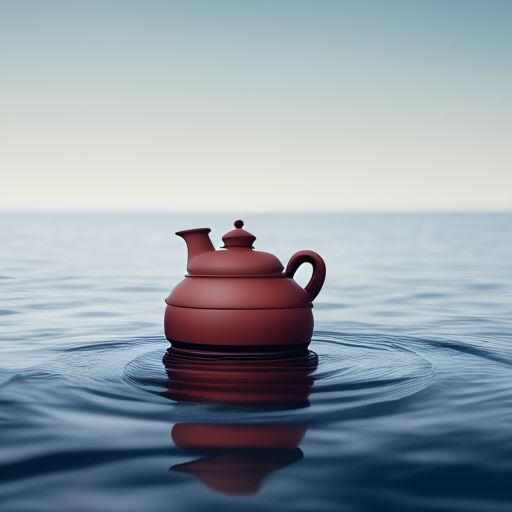
\includegraphics[width=\xwidth]{cp2/figures/dreambooth/teapot/c320_checkpoint_99.png} &
    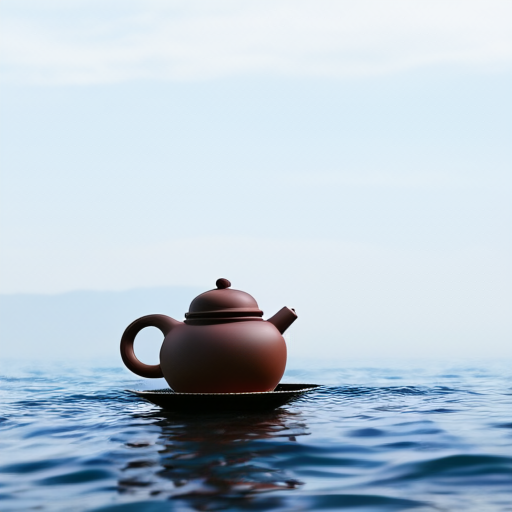
\includegraphics[width=\xwidth]{cp2/figures/dreambooth/teapot/c512_checkpoint_499.png} \\
    Inputs & \texttt{430M} &  \texttt{558M} &  \texttt{866M} &  \texttt{2B} \\
    \\
    &
    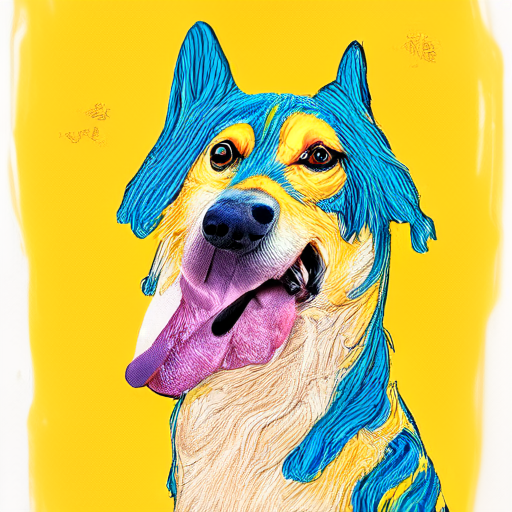
\includegraphics[width=\xwidth]{cp2/figures/dreambooth/dog/c96_checkpoint_99.png} &
    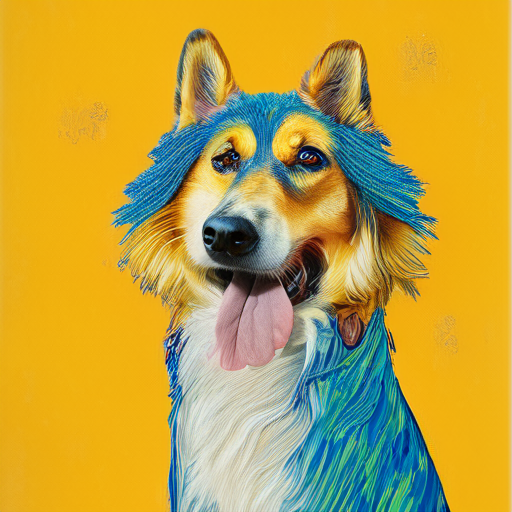
\includegraphics[width=\xwidth]{cp2/figures/dreambooth/dog/c128_checkpoint_99.png} &
    \includegraphics[width=\xwidth]{cp2/figures/dreambooth/dog/c160_checkpoint_99.png} &
    \includegraphics[width=\xwidth]{cp2/figures/dreambooth/dog/c192_checkpoint_99.png} \\
    &  \texttt{83M} &  \texttt{145M} &  \texttt{223M} &  \texttt{318M} \\
    \multirow[t]{3}{*}{
    \includegraphics[width=0.3\linewidth]{cp2/figures/dreambooth/dog/dog.pdf}
    } &
    \includegraphics[width=\xwidth]{cp2/figures/dreambooth/dog/c224_checkpoint_99.png} &
    \includegraphics[width=\xwidth]{cp2/figures/dreambooth/dog/c256_checkpoint_99.png} &
    \includegraphics[width=\xwidth]{cp2/figures/dreambooth/dog/c320_checkpoint_99.png} &
    \includegraphics[width=\xwidth]{cp2/figures/dreambooth/dog/c512_checkpoint_99.png} \\
    Inputs &  \texttt{430M} &  \texttt{558M} &  \texttt{866M} &  \texttt{2B} \\
    
    \end{tabular}
    \caption{
    Visualization of the Dreambooth results (using 50-step DDIM sampling and CFG rate of 7.5) shows two distinct tiers based on model size.  Smaller models (\texttt{83M}-\texttt{223M}) perform similarly, as do larger ones (\texttt{318M}-\texttt{2B}),  with a clear quality advantage for the larger group.
    }
    %
    %In subject-driven text-to-image synthesis (Dreambooth), we observe that the visual quality of results between different model sizes can be grouped by small (\texttt{83M}, \texttt{145M}, \texttt{223M}) and large models (\texttt{318M}, \texttt{430M}, \texttt{558M}, \texttt{866M}, \texttt{2B}). The difference between models in the same group is relatively small.}
    \label{fig:dreambooth}
\end{figure*}

\subsection{Pretraining scales downstream performance}
\label{sec:scalingsr}
Using scaled models based on their pretraining on text-to-image data, we finetune these models on the downstream tasks of real-world super-resolution~\cite{saharia2022image, sahak2023denoising} and DreamBooth~\cite{ruiz2023dreambooth}.
The performance of these pretrained models is shown in Table.~\ref{tab:scaling_config}.
In the left panel of Fig.~\ref{fig:sr_compute}, we present the generative performance FID versus training compute on the super-resolution (SR) task.
It can be seen that the performance of SR models is more dependent on the model size than training compute.
%Our results indicate that smaller models, even when trained for extended periods, can not achieve a comparable performance of larger models.
Our results demonstrate a clear limitation of smaller models: they cannot reach the same performance levels as larger models, regardless of training compute.

While the distortion metric LPIPS shows some inconsistencies compared to the generative metric FID (Fig.~\ref{fig:sr_compute}), Fig.~\ref{fig:sr} clearly demonstrates that larger models excel in recovering fine-grained details compared to smaller models.
% We suspect the inconsistency between the generative metric FId and the distortion metric LPIPS is resulted by the text-to-image pretraining used in super-resolution.

The key takeaway from Fig.~\ref{fig:sr_compute} is that large super-resolution models achieve superior results even after short finetuning periods compared to smaller models. This suggests that pretraining performance (dominated by the pretraining model sizes) has a greater influence on the super-resolution FID scores than the duration of finetuning (\ie, training compute for finetuning).


% Specifically, the FID score (left panel of Fig.~\ref{fig:sr_compute}) in super-resolution has a similar trend as the one in text-to-image pretraining, where larger model achieve better performance.
% The similar trend suggests that the FID score of super-resolution may be denominated by the pretraining, while the pretraining may have less effects on the distortion metric LPIPS, and hence these two metrics show inconsistency trends when scaling training compute.

%Although the distortion metric, i.e., LPIPS, displayed in the right panel of Figure~\ref{fig:sr_compute}, exhibits inconsistent trends compared to the generative metric FID, we highlights that larger models are indeed capable of recovering more fine-grained details than smaller models, as illustrated in Figure~\ref{fig:sr}.
Furthermore, we compare the visual results of the DreamBooth finetuning on the different models in Fig.~\ref{fig:dreambooth}. We observe a similar trend between  visual quality and  model size.


\subsection{Scaling sampling-efficiency}

\begin{figure}[!t]
    \centering
    \begin{subfigure}[b]{\linewidth}
    \includegraphics[width=\linewidth]{cp2/figures/145M_cfg.jpg}
    \caption{50-step sampling results of the 145M model}
    \end{subfigure}
    \begin{subfigure}[b]{\linewidth}
    \includegraphics[width=\linewidth]{cp2/figures/866M_cfg.jpg}
    \caption{50-step sampling results of the 866M model}
    \end{subfigure}
    \caption{Visualization of text-to-image results with 50-step DDIM sampling and different CFG rates (from left to right in each row: $(1.5, 2.0, 3.0, 4.0, 5.0, 6.0, 7.0, 8.0)$). The prompt used is ``\emph{A raccoon wearing formal clothes, wearing a top hat and holding a cane. Oil painting in the style of Rembrandt.}''.
    We observe that changes in CFG rates impact visual quality more significantly than the prompt semantic accuracy.
    We use the FID score for quantitative determination of optimal sampling performance (Fig.~\ref{fig:cfgrate}) because it directly measures visual quality, unlike the CLIP score, which focuses on semantic similarity. }
    \label{fig:cfgratevisual}
    \vspace{-1\baselineskip}
\end{figure}

\begin{figure}[t]
    \centering
    \includegraphics[width=\linewidth]{cp2/figures/analyze_cfg_rates_v4.pdf}
    \vspace{-1.5\baselineskip}
    \caption{
    The impact of the CFG rate on text-to-image generation depends on the model size and sampling steps. As demonstrated in the left and center panels, the optimal CFG rate changes as the sampling steps increased.
    %two models of different sizes exhibit contrasting performance under varying CFG rates. 
    To determine the optimal performance (according to the FID score) of each model and each sampling steps, we systematically sample the model at various CFG rates and identify the best one. As a reference of the optimal performance, the right panel shows the CFG rate corresponding to the optimal performance of each model for a given number of sampling steps.
    }
    \label{fig:cfgrate}
\end{figure}

\subsubsection{Analyzing the effect of CFG rate.}
\label{sec:optimalparams}


%Given the fact that the performance of generative models can hardly be measured by a single metric, the sampling parameters play a crucial role in controlling different properties of the generated results, especially the Classifier-Free Guidance (CFG) rate~\cite{ho2022classifier} that balances the visual quality and the semantic accuracy of generated results.
Text-to-image generative models require nuanced evaluation beyond single metrics. Sampling parameters are vital for customization, with the Classifier-Free Guidance (CFG) rate~\cite{ho2022classifier} directly influencing the balance between visual fidelity and semantic alignment with text prompt. Rombach et al.~\cite{rombach2022high} experimentally demonstrate that different CFG rates result in different CLIP and FID scores.


\begin{figure}[!t]
    \centering 
    \def\xwidth{.3\linewidth}
    \includegraphics[height=\xwidth]{cp2/figures/analyze_inference_steps_costs.pdf}
    \includegraphics[height=\xwidth]{cp2/figures/analyze_inference_costs.pdf}
    \vspace{-.5\baselineskip}
    \caption{%
    Comparison of text-to-image performance of models with varying sizes. The left figure shows the relationship between sampling cost (normalized cost $\times$ sampling steps) and sampling steps for different model sizes. The right figure plots the optimal text-to-image FID score among CFG rates of $(1.5, 2.0, 3.0, 4.0, 5.0, 6.0, 7.0, 8.0)$ as a function of the sampling cost for the same models.
    Key Observation: Smaller models achieve better FID scores than larger models for a fixed sampling cost. For instance, at a cost of 3, the 83M model achieves the best FID compared to the larger models. This suggests that smaller models can be more efficient in achieving good results with lower costs.
    }
    \label{fig:optiamlrules}
    % \vspace{-1\baselineskip}
\end{figure}


\begin{figure}[!ht]
    \centering
    \def\xwidth{.24\linewidth}
    % \begin{subfigure}[b]{\linewidth}
    % \imageWithNote{\xwidth}{\scriptsize \raggedleft \texttt{83M\,}}{cp2/figures/efficiency/c96_0_step_50_5.0.jpg}
    % \imageWithNote{\xwidth}{\scriptsize \raggedleft \texttt{145M}}{cp2/figures/efficiency/c128_0_step_50_3.0.jpg}
    % \imageWithNote{\xwidth}{\scriptsize \raggedleft \texttt{223M}}{cp2/figures/efficiency/c160_0_step_20_3.0.jpg}
    % \imageWithNote{\xwidth}{\scriptsize \raggedleft \texttt{318M}}{cp2/figures/efficiency/c192_0_step_10_4.0.jpg}
    % \hfill
    
    % \imageWithNote{\xwidth}{\scriptsize \raggedleft \texttt{430M}}{cp2/figures/efficiency/c224_0_step_8_5.0.jpg}
    % \imageWithNote{\xwidth}{\scriptsize \raggedleft \texttt{558M}}{cp2/figures/efficiency/c256_0_step_6_6.0.jpg}
    % \imageWithNote{\xwidth}{\scriptsize \raggedleft \texttt{704M}}{cp2/figures/efficiency/c288_0_step_6_6.0.jpg}
    % \imageWithNote{\xwidth}{\scriptsize \raggedleft \texttt{866M}}{cp2/figures/efficiency/c320_0_step_4_8.0.jpg}
    % \vspace{.5em}
    % \caption{Prompt: \emph{``A corgi's head depicted as a nebula.''}. Sampling Cost $\approx$ 6.}
    % \end{subfigure}
     \begin{subfigure}[b]{\linewidth}
    \imageWithNote{\xwidth}{\scriptsize \raggedleft \texttt{83M\,}}{cp2/figures/t2i-efficiency/0_step_50_6.0.jpg}
    \imageWithNote{\xwidth}{\scriptsize \raggedleft \texttt{145M}}{cp2/figures/t2i-efficiency/0_step_45_8.0.jpg}
    \imageWithNote{\xwidth}{\scriptsize \raggedleft \texttt{223M}}{cp2/figures/t2i-efficiency/0_step_40_6.0.jpg}
    \imageWithNote{\xwidth}{\scriptsize \raggedleft \texttt{318M}}{cp2/figures/t2i-efficiency/0_step_35_4.0.jpg}
    \hfill
    
    \imageWithNote{\xwidth}{\scriptsize \raggedleft \texttt{430M}}{cp2/figures/t2i-efficiency/0_step_30_7.0.jpg}
    \imageWithNote{\xwidth}{\scriptsize \raggedleft \texttt{558M}}{cp2/figures/t2i-efficiency/0_step_20_6.0.jpg}
    \imageWithNote{\xwidth}{\scriptsize \raggedleft \texttt{704M}}{cp2/figures/t2i-efficiency/0_step_4_7.0.jpg}
    \imageWithNote{\xwidth}{\scriptsize \raggedleft \texttt{866M}}{cp2/figures/t2i-efficiency/0_step_4_8.0.jpg}
    \vspace{.5em}
    \caption{Prompt: \emph{``A corgi's head depicted as a nebula.''}. Sampling Cost $\approx$ 6.}
    \end{subfigure}
    \vspace{1em}
    \begin{subfigure}[b]{\linewidth}
    
    \imageWithNote{\xwidth}{\scriptsize \raggedleft \texttt{83M\,}}{cp2/figures/efficiency/c96_1_step_50_5.0.jpg}
    \imageWithNote{\xwidth}{\scriptsize \raggedleft \texttt{145M}}{cp2/figures/efficiency/c128_1_step_50_7.0.jpg}
    \imageWithNote{\xwidth}{\scriptsize \raggedleft \texttt{223M}}{cp2/figures/t2i-efficiency-2/1_step_50_8.0.jpg}
    \imageWithNote{\xwidth}{\scriptsize \raggedleft \texttt{318M}}{cp2/figures/t2i-efficiency-2/1_step_45_7.0.jpg}
    \hfill
    
    \imageWithNote{\xwidth}{\scriptsize \raggedleft \texttt{430M}}{cp2/figures/efficiency/c224_1_step_20_4.0.jpg}
    \imageWithNote{\xwidth}{\scriptsize \raggedleft \texttt{558M}}{cp2/figures/efficiency/c256_1_step_20_4.0.jpg}
    \imageWithNote{\xwidth}{\scriptsize \raggedleft \texttt{704M}}{cp2/figures/efficiency/c288_1_step_20_4.0.jpg}
    \imageWithNote{\xwidth}{\scriptsize \raggedleft \texttt{866M}}{cp2/figures/efficiency/c320_1_step_10_6.0.jpg}
    \vspace{.5em}
    \caption{Prompt: \emph{``A pineapple surfing on a wave.''}. Sampling Cost $\approx$ 12.}
    \end{subfigure}
    \vspace{-2\baselineskip}
    \caption{Text-to-image results of the scaled LDMs under approximately the same inference cost (normalized cost $\times$ sampling steps). Smaller models can produce comparable or even better visual results than larger models under similar sampling cost.
    % Empirically, 1 sampling cost equals to 100 ms running time on TPUv5.
    % The results suggests that by scaling down LDMs into smaller model sizes, we can even 
    % The results suggest that LDM can generate reasonable results in around 0.6 second (6 sampling cost) on TPUv5 by scaling down.
    }
    \label{fig:optimalvisual}
    \vspace{-1\baselineskip}
\end{figure}

\begin{figure}[ht]
    \centering
    \def\xwidth{.3\linewidth}
     \includegraphics[height=\xwidth]{cp2/figures/ddpm_analyze_inference_costs_B.pdf}
    \includegraphics[height=\xwidth]{cp2/figures/dpmsolver_plus_plus_analyze_inference_costs_B.pdf}
    \vspace{-.5\baselineskip}
    \caption{\emph{Left}: Text-to-image performance FID as a function of the sampling cost (normalized cost $\times$ sampling steps) for the DDPM sampler (solid curves) and the DDIM sampler (dashed curves). \emph{Right}: Text-to-image performance FID as a function of the sampling cost for the second-order DPM-Solver++ sampler (solid curves) and the DDIM sampler (dashed curves). Suggested by the trends shown in Fig.~\ref{fig:optiamlrules}, we only show the sampling steps $\leq 50$ as using more steps does not improve the performance.}
    \label{fig:scalingsampler}
    \vspace{-1\baselineskip}
\end{figure} 


In this study, we find that CFG rate as a sampling parameter yields inconsistent results across different model sizes.
Hence, it is interesting to quantitatively determine the \textit{optimal} CFG rate for each model size and sampling steps using either FID or CLIP score.
We demonstrate this by sampling the scaled models using different CFG rates, \ie, $(1.5, 2.0, 3.0, 4.0, 5.0, 6.0, 7.0, 8.0)$ and comparing their quantitative and qualitative results. 
%
%
In Fig.~\ref{fig:cfgratevisual}, we present visual results of two models under varying CFG rates, highlighting the impact on the visual quality. We observed that changes in CFG rates impact visual quality more significantly than prompt semantic accuracy and therefore opted to use the FID score for quantitative determination of the optimal CFG rate. performance. Fig.~\ref{fig:cfgrate} shows how different classifier-free guidance rates affect the FID scores in text-to-image generation (see figure caption for more details). 


\subsubsection{Scaling efficiency trends.}
\label{sec:optimalmodelsizes}

Using the optimal CFG rates established for each model at various number of sampling steps, we analyze the optimal performance to understand the sampling efficiency of different LDM sizes.
%Leveraging the previously determined optimal CFG rates for each model when different number of sampling steps are used, we analize the optimal performance for revealing the sampling efficiency across different sizes of LDMs.
%
% Such an analysis can reveal the sampling efficiency across different model sizes of LDMs, by checking the lowest curve that crosses the vertical line started by the sampling cost, it is easy to determine the optimal model sizes.
% Such analysis can reveal the sampling efficiency across different sizes of LDMs, with the most efficient model size identifiable by the lowest curve intersecting a vertical line that denotes the sampling cost.
%
Specifically, in Fig.~\ref{fig:optiamlrules}, we present a comparison between different models and their optimal performance given the sampling cost (normalized cost $\times$ sampling steps).
By tracing the points of optimal performance across various sampling cost---represented by the dashed vertical line---we observe a consistent trend: smaller models frequently outperform larger models across a range of sampling cost in terms of FID scores.
Furthermore, to visually substantiate better-quality results generated by smaller models against larger ones, Fig.~\ref{fig:optimalvisual} compares the results of different scaled models, which highlights that the performance of smaller models can indeed match their larger counterparts under similar sampling cost conditions.
\emph{
Please see our supplement for more visual comparisons.
}

\subsection{Scaling sampling-efficiency in different samplers}
\label{sec:samplerscaling}

To assess the generalizability of observed scaling trends in sampling efficiency, we compared scaled LDM performance using different diffusion samplers. In addition to the default DDIM sampler, we employed two representative alternatives: the stochastic DDPM sampler~\cite{ho2020denoising} and the high-order DPM-Solver++~\cite{lu2022dpm2}.

Experiments illustrated in Fig.~\ref{fig:scalingsampler} reveal that the DDPM sampler typically produces lower-quality results than DDIM with fewer sampling steps, while the DPM-Solver++ sampler generally outperforms DDIM in image quality (see the figure caption for details).
%
Importantly, we observe consistent sampling-efficiency trends with the DDPM and DPM-Solver++ sampler as seen with the default DDIM: smaller models tend to achieve better performance than larger models under the same sampling cost. Since the DPM-Solver++ sampler is not designed for use beyond 20 steps, we focused our testing within this range.
%
This finding demonstrates that the scaling properties of LDMs remain consistent regardless of the diffusion sampler used.
%


\subsection{Scaling downstream sampling-efficiency}
\label{sec:scalingsamplingsr}


\begin{figure}[t]
    \centering
    \def\xwidth{.315\linewidth}
    \includegraphics[height=\xwidth]{cp2/figures/sr_fid_cost_l_20steps.pdf}
    \includegraphics[height=\xwidth]{cp2/figures/sr_fid_cost_g_50steps.pdf}
    \vspace{-1.5\baselineskip}
    \caption{Super-resolution performance vs. sampling cost for different model sizes. \emph{Left:} FID scores of super-resolution models under limited sampling steps (less than or equal to 20). Smaller models tend to achieve lower (better) FID scores within this range.
    \emph{Right:} FID scores of super-resolution models under a larger number of sampling steps (greater than 20).
    Performance differences between models become less pronounced as sampling steps increase.
%
%    \emph{Left}: $4\times$ real super-resolution FID score as a function of the sampling cost (normalized cost $\times$ sampling steps) for different models, tested under sampling steps are less or equal than 20 sampling steps.
%    \emph{Right} Super-resolution performance FID as a function of the sampling cost for different models, tested under sampling steps are greater than 20 sampling steps.
    }
    \label{fig:sroptiamlrules}
    \vspace{-1\baselineskip}
\end{figure}


Here, we investigate the scaling sampling-efficiency of LDMs on downstream tasks, specifically focusing on the super-resolution task.
Unlike our earlier discussions on optimal sampling performance, there is limited literature demonstrating the positive impacts of SR performance without using classifier-free guidance.
Thus, our approach directly uses the SR sampling result without applying classifier-free guidance.
Inspired from Fig.~\ref{fig:sr_compute}, where the scaled downstream LDMs have significant performance difference in 50-step sampling, we investigate sampling efficiency from two different aspects, \ie, fewer sampling steps $[4, 20]$ and more sampling steps $(20, 250]$. 
As shown in the left part of Fig.~\ref{fig:sroptiamlrules}, the scaling sampling-efficiency still holds in the SR tasks when the number of sampling steps is less than or equal to 20 steps.
Beyond this threshold, however, larger models demonstrate greater sampling-efficiency than smaller models, as illustrated in the right part of Fig.~\ref{fig:sroptiamlrules}.
This observation suggests the consistent sampling efficiency of scaled models on fewer sampling steps from text-to-image generation to super-resolution tasks.

\begin{figure}[!t]
    \centering
    \def\xwidth{.31\linewidth}
    \includegraphics[height=\xwidth]{cp2/figures/analyze_distill_perfomrance.pdf}
    \includegraphics[height=\xwidth]{cp2/figures/analyze_distill_inference_costs.pdf}
    \vspace{-.5\baselineskip}
    \caption{Distillation improves text-to-image performance and scalability. \emph{Left:} Distilled Latent Diffusion Models (LDMs) consistently exhibit lower (better) FID scores compared to their undistilled counterparts across varying model sizes. The consistent acceleration factor (approx. $5\times$) indicates that the benefits of distillation scale well with model size.
    \emph{Right:} Distilled models using only 4 sampling steps achieve FID scores comparable to undistilled models using significantly more steps. Interestingly, at a sampling cost of 7, the distilled \texttt{866M} model performs similarly to the smaller, undistilled \texttt{83M} model, suggesting improved efficiency. 
    % \emph{See the supplement for visual examples after distillation.}
    }
    \label{fig:distll}
    \vspace{-1\baselineskip}
\end{figure}


\subsection{Scaling sampling-efficiency in distilled LDMs.}
\label{sec:scalingdistill}

We have featured the scaling sampling-efficiency of latent diffusion models, which demonstrates that smaller model sizes exhibit higher sampling efficiency.
A notable caveat, however, is that smaller models typically imply reduced modeling capability. This poses a challenge for recent diffusion distillation methods~\cite{luhman2021knowledge, salimans2022progressive, song2023consistency, sauer2023adversarial, gu2023boot, mei2023conditional,luo2023latent, lin2024sdxl} that heavily depend on modeling capability.
One might expect a contradictory conclusion and believe the distilled large models sample faster than distilled small models.
In order to demonstrate the sampling efficiency of scaled models after distillation, we distill our previously scaled models with conditional consistency distillation~\cite{song2023consistency, mei2023conditional} on text-to-image data and compare those distilled models on their optimal performance.
% \emph{Please see our supplement for more distillation details.}

To elaborate, we test all distilled models with the same 4-step sampling, which is shown to be able to achieve the best sampling performance; we then compare each distilled model with the undistilled one on the normalized sampling cost.
We follow the same practice discussed in Section~\ref{sec:optimalparams} for selecting the optimal CFG rate and compare them under the same relative inference cost.
The results shown in the left part of Fig.~\ref{fig:distll} demonstrate that distillation significantly improves the generative performance for all models in 4-step sampling, with FID improvements across the board.
% Furthermore, by comparing these distilled models on the normalized sampling cost for 4-step sampling, the right part of Figure~\ref{fig:distll} shows that smaller models can still achieve the compared performance as the larger distilled models with the same sampling cost. 
By comparing these distilled models with the undistilled models in the right part of Fig.~\ref{fig:distll}, we demonstrate that distilled models outperform undistilled models at the same sampling cost.
However, at the specific sampling cost, \ie, sampling cost $\approx \texttt{8}$, the smaller undistilled 83M model still achieves similar performance to the larger distilled 866M model.
%
The observation further supports our proposed scaling sampling-efficiency after diffusion distillation.


\section{Conclusion}
In this paper, we investigated scaling properties of Latent Diffusion Models (LDMs), specifically through scaling model size from 39 million to 5 billion parameters.
We trained these scaled models from scratch on a web-scale text-to-image dataset and then finetuned the pretrained models for downstream tasks.
Our findings unveil that, under identical sampling costs, smaller models frequently outperform larger models, suggesting a promising direction for accelerating LDMs in terms of model size.
We further show that the sampling efficiency is consistent in multiple axes. For example, it is invariant to various diffusion samplers (stochastic and deterministic), and also holds true for distilled models.
We believe this analysis of scaling sampling efficiency would  be instrumental in guiding future developments of LDMs, specifically for balancing model size against performance and efficiency in a broad spectrum of practical applications.
